% load lecture note class
\documentclass{notesclass}
\begin{document}
\begin{titlepage}
    \university{University of Stavanger}
    \courseid{DAT550}
    \title{Summary of lecture notes}
    \author{Håvard Godal}
    \version{Spring 2021}
    \maketitle
\end{titlepage}

{
  \hypersetup{linkcolor=black}
  \tableofcontents
}


\chapter{Introduction to Data Mining}
\section{Data}
Data is units of information, and in a technical perspective, data is a set
of values of quantitative or qualitative variables about a data object. 
Data should be understood in the context of information. Information can be 
thought of as the resolution of uncertainty, though it's 
exact interpretation and meaning differs in different context. Using this
vague definition of information it becomes clear how diverse data can be.
Everything that removes uncertainty contains information and can potentially 
be stored and processed as data. Examples of data can be 

\begin{itemize}
    \item Tabular Data like spreadsheets.
    \item A news article.
    \item A photograph.
    \item A TV broadcast.
    \item And much much more.
\end{itemize}

Historically, computation has been done on numerical data like tabulated data,
but in the later decades data mining and machine learning methods have broadened
what data algorithms can use to do inference. One example is Neural Networks
and image classification.

\section{Data Mining}
Data mining can be described as:

\begin{center}
    \textit{"Non-trivial extraction of implicit, \\
    previously unknown and potential useful information from data"}
\end{center}

\begin{center}
    \textit{"Exploration and analysis, by automatic or semi-automatic means, \\
    of large quantities of data in order to discover meaningful patterns"}
\end{center}

Data mining is a process of extracting 
and discovering patterns in large data sets involving methods at the 
intersection of machine learning, statistics, and database systems. 
Data mining is an interdisciplinary subfield of computer science and statistics 
with an overall goal to extract information (with intelligent methods) 
from a data set and transform the information into a comprehensible structure 
for further use. \cite{enwiki:datamining}

\section{Machine Learning}

Machine learning can be described as:

\begin{center}
    \textit{"The field of study that gives computers the ability to learn \\
    without being explicitly programmed"}
\end{center}

\begin{center}
    \textit{"A computer program is said to learn from experience E \\
     with respect to some class of tasks T and performance measure P, \\
     if its performance at tasks in T, as measured by P, improves with experience E"}
\end{center}

Machine learning (ML) is the study of computer algorithms that improve 
automatically through experience and by the use of data. It is seen as a part of 
artificial intelligence. Machine learning algorithms build a model based on 
sample data, known as "training data", in order to make predictions or decisions 
without being explicitly programmed to do so. Another way to think about it as 
an abstract mathematical formula.

\begin{equation}
    f: \text{input} \rightarrow \text{output}
\end{equation}

The abstract function $f$ can be any regression-, classification-, association
or calculation problem or anything else that can be thought of as the formula
above. In traditional programming, the programmer has collected the input
and manually created $f$ and get the output of interest. I.e. the programmer
collects input, the rules $f$ and calculates the output. In machine learning, 
the programmer have access to the input and the output 
and the computer estimates $f$. I.e. the programmer collects inputs and outputs
and uses the computer to find the rules. 

\newpage
\section{Data Mining or Machine Learning}

Data mining is the process of discovering patterns in large data sets involving methods at the interseciton of machine learning, statistics, and database systems.
\begin{figure}[H]
    \centering
    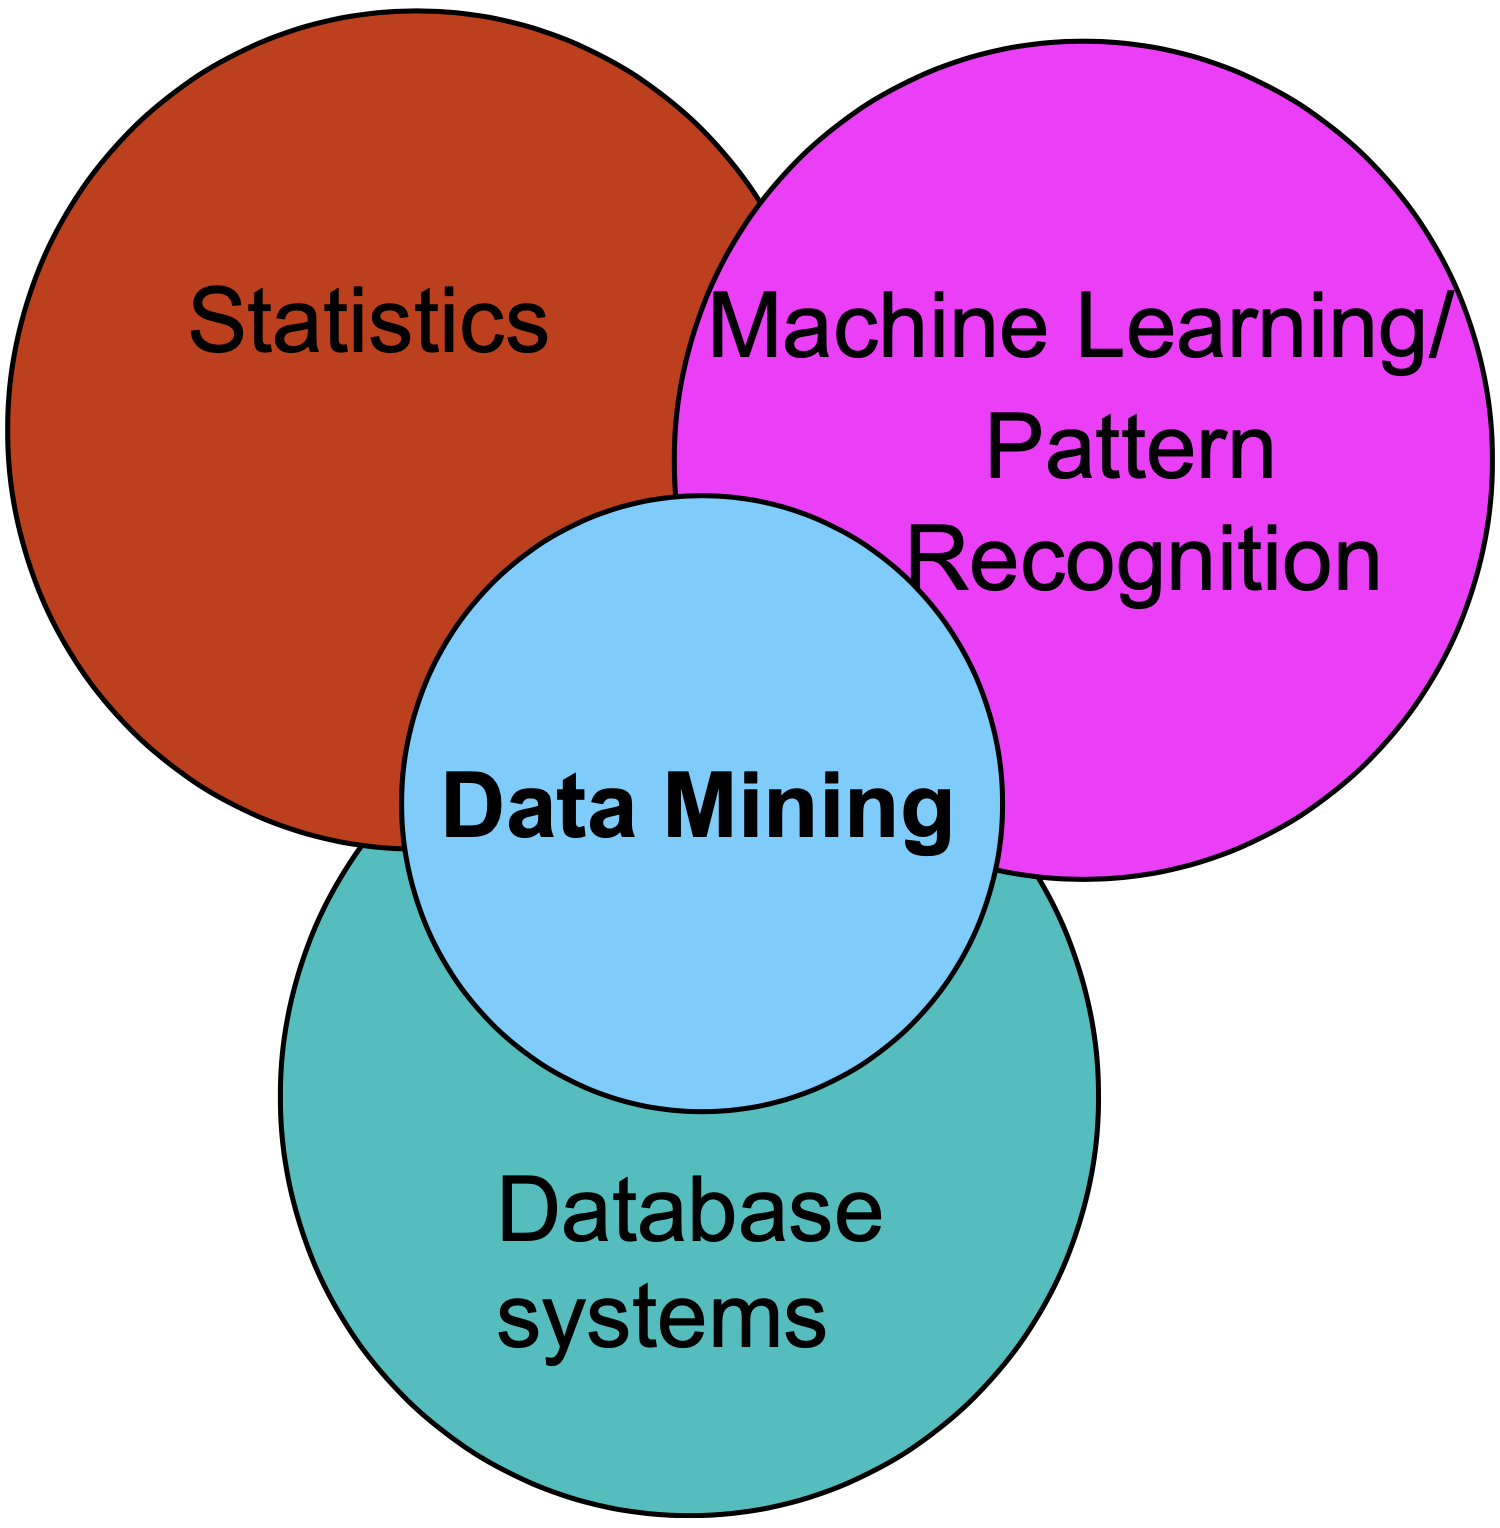
\includegraphics[scale=0.2]{figures/datamining.png}
    \caption{Diagram of Data Mining}
\end{figure}


\section{Properties of Data Mining}
\subsection{Commercial viewpoint}
Lots of data is being collected and warehoused, such as web data, purchases, and transactions.
Computation power has become cheap and powerful, and the competitive pressure is strong.
It is therefore necessary to provide better, customized servicees for an edge.

\subsection{Scientific Viewpoint}
Data is collected and stored at enormous speeds, up to multiple terrabytes per hour.
Such data can be generated from the large hydron collider and from scanning the universe.
Such data can not be interpreted by traditional techniques, and requires data mining to classify and segment the data,
and form hypothesis formations.

\newpage
\subsection{KDD Process}
Knowledge Discovery in Databases (KDD) refers to the overall process of discovering useful knowledge from data.

KDD is an integration of multiple technologies for data management such as database management and data warehousing, 
statistic machine learning, decision support, and others such as visualisation and parallel computing. 

\begin{figure}[H]
    \centering
    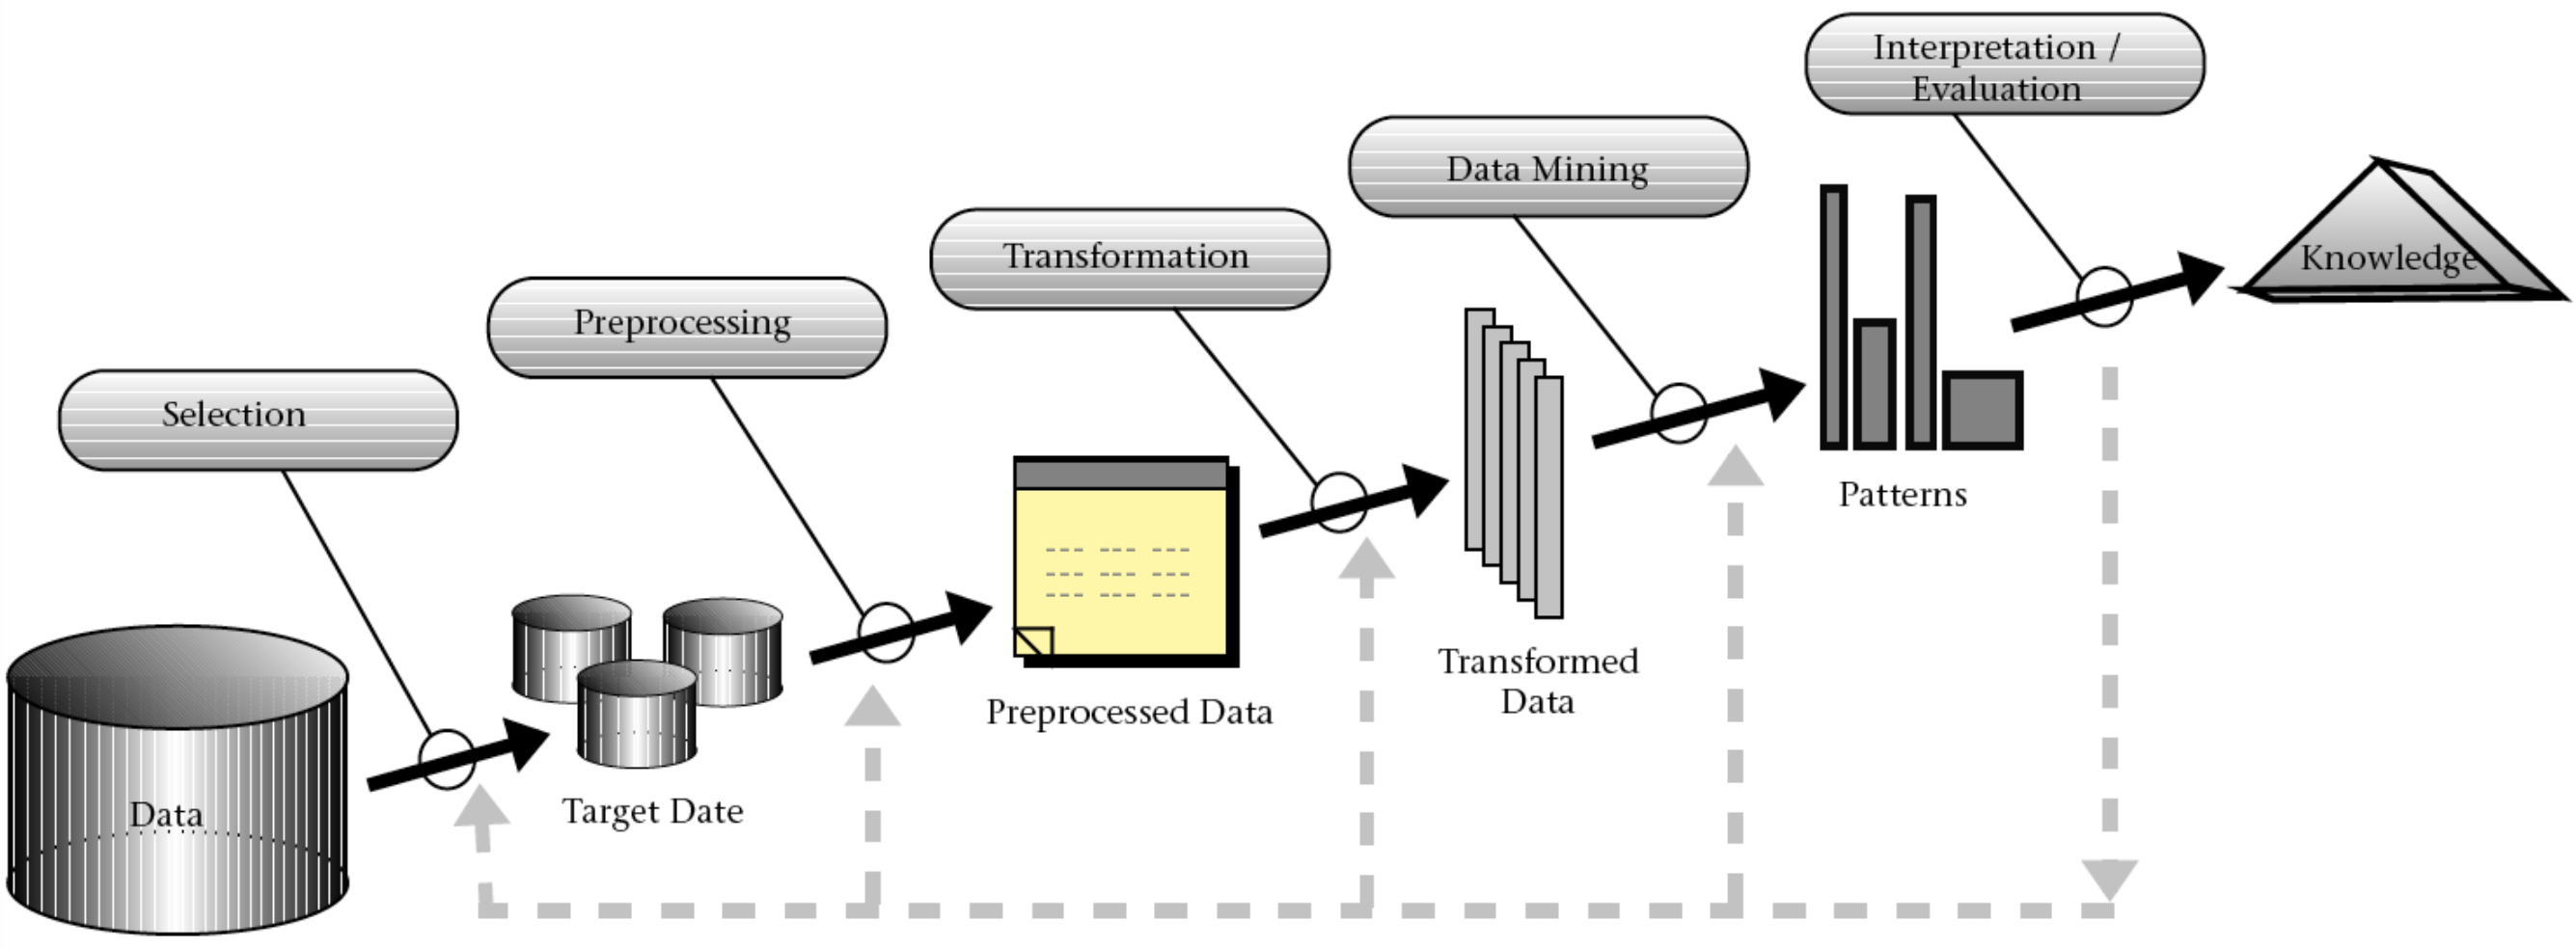
\includegraphics[scale=0.2]{figures/kdd.png}
    \caption{The KDD Process}
\end{figure}

\section{Data Mining tasks}
\begin{itemize}
    \item Prediction methods
    \begin{itemize}
        \item Use some variables to predict unknown or future values of other variables.
        \begin{itemize}
            \item Supervised (classification or regression)
            \item Unsupervised (clustering)
            \item Semi-supervised
        \end{itemize}
    \end{itemize}
    \item Descriptive methods
    \begin{itemize}
        \item Find human-interpretable patterns that describe the data.
        \begin{itemize}
            \item Rule mining
            \item Frequent patterns
            \item Anomaly detection
        \end{itemize}
    \end{itemize}
\end{itemize}

\section{Regression}
\begin{enumerate}
    \item Given a set of data points/instances along with “correct” answers or 
    labels (training data)
    \item Feed it to an algorithm which can learn a model and predict the 
    correct value for an unseen data point (test data)
    \item The learned model is an approximate representation of the training 
    data
    \item Predict continuous valued output (price in the previous example)
    \item The algorithm should produce more right answers (goal)
\end{enumerate}

\section{Unsupervised Learning}
\begin{itemize}
    \item Unsupervised learning includes unlabeled data
    \item One way of doing this would be to cluster data into to groups
    \begin{itemize}
        \item Group data points which are similar together, while separating 
        dissimilar items as much as possible
        \item This is a clustering algorithm
    \end{itemize}
\end{itemize}

\section{Association Rule Mining}
\begin{itemize}
    \item Given a set of records each of which contain some number of items from a given collection
    \item Produce dependency rules which will predict occurrence of an item based on occurrences of other items
\end{itemize}
Such rules can be used for marketing and sales promotion. Rule mining can also be used for inventory management, and much more.

\section{Challenges in Data Mining}
\begin{itemize}
    \item Scalability
    \item Dimensionality
    \item Heterogenous or complex data
    \item Data ownership and distribution
    \item Privacy concern
    \item Data quality
    \item Evolving/streaming data
\end{itemize}



\chapter{Data}
\section{Data Recap}

\begin{figure}
    \centering
    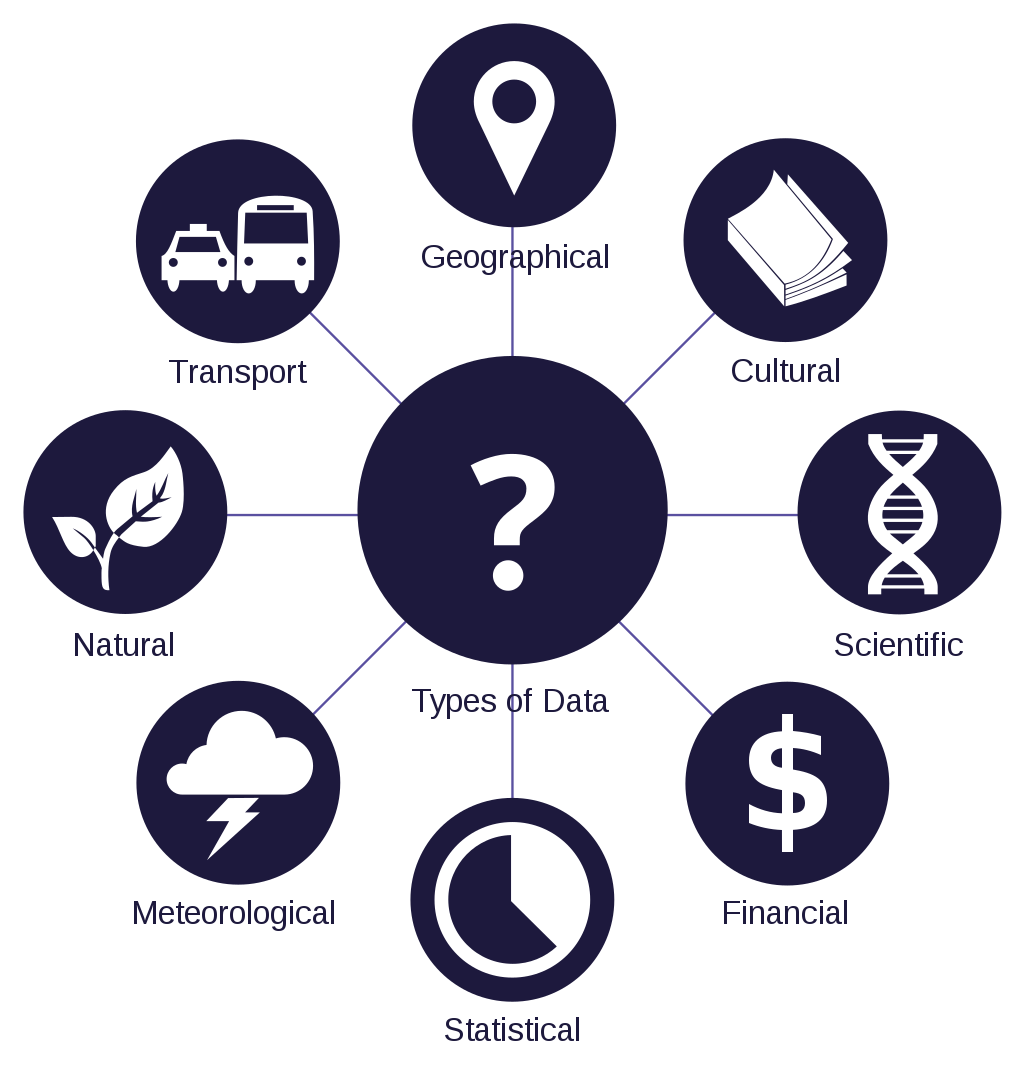
\includegraphics[width=0.5\linewidth]{figures/datatypespng.png}
    \caption{Different kinds of data.}
    \label{fig:datatypes}
\end{figure}

Data is units of information, and in a technical perspective, data is a set
of values of quantitative or qualitative variables about a data object. 
Data should be understood in the context of information. Information can be 
thought of as the resolution of uncertainty, though it's 
exact interpretation and meaning differs in different context. Using this
vague definition of information it becomes clear how diverse data can be.
Just see figure \ref{fig:datatypes} for examples. 
Everything that removes uncertainty contains information and can potentially 
be stored and processed as data.

\subsection{Difference between data and information.}
Data and Information is often talked about interchangably but are two different
things or rather two different levels of abstraction of the same thing. Data is 
a structured or unstructured collection of symbols. Information resolves 
uncertainty and does not take any particular form. Data can represent reduntant
symbols but can be said to approach information through optimal compression. 
One of the most common ways to structure data is to have a set of data objects
and their attributes.

\section{Attributes}
\begin{itemize}
    \item An attribute is a property or characteristic of an object
    \begin{itemize}
        \item Attribute are also known as variables, fields, characteristics, or features
    \end{itemize}
    \item A collection of attributes describe an object
    \begin{itemize}
        \item Objects are also known as records, points, cases, samples, entries, or instances
    \end{itemize}
\end{itemize}

\subsection{Values}
Attribute values are numbers or symbols assigned to an attribute.
The distinction between attributes and attribute values are:
\begin{itemize}
    \item Same attribute can be mapped to different attribute values
    \item Different attributes can be mapped to the same set of values
\end{itemize}

\subsection{Types}
\begin{center}
    \begin{table}[H]
        \begin{tabular}{l|l|l}
            \begin{tabular}[c]{@{}l@{}}
                Attribute \\Type
            \end{tabular}&
            Operations &
            Transformations \\ \hline \hline
        \begin{tabular}[c]{@{}l@{}}
            \\Nomial\\ \\
        \end{tabular}&
            \begin{tabular}[c]{@{}l@{}}
                Mode, Entropy, Contingency, \\
                Correlation, $\chi^2$-test
            \end{tabular}&
            \begin{tabular}[c]{@{}l@{}}
                Any permutation of values
            \end{tabular} \\ \hline
        \begin{tabular}[c]{@{}l@{}}
            \\Ordinal\\ \\
        \end{tabular}&
            \begin{tabular}[c]{@{}l@{}}
                Median, Rank correlation, \\
                Percentiles, Run tests, Sign tests
            \end{tabular}&
            \begin{tabular}[c]{@{}l@{}}
                Order-preserving change of values\\
                $new\_value = f(old\_value)$ \\
                where $f$ is a monotonic function.
            \end{tabular} \\ \hline
        \begin{tabular}[c]{@{}l@{}}
            \\Interval\\ \\
        \end{tabular}&
            \begin{tabular}[c]{@{}l@{}}
                Mean, Standard deviation, $t$-tests\\
                Pearson's correlation, $F$-tests
            \end{tabular}&
            \begin{tabular}[c]{@{}l@{}}
                $new\_value = a * old\_value + b$ \\
                where a and b are constants
            \end{tabular} \\ \hline
        \begin{tabular}[c]{@{}l@{}}
            \\Ratio\\ \\
        \end{tabular}&
            \begin{tabular}[c]{@{}l@{}}
                Geometric mean, Harmonic mean, \\
                Percent variation
            \end{tabular}&
            \begin{tabular}[c]{@{}l@{}}
                $new\_value = a * old\_value$
            \end{tabular}
        \end{tabular}
    \end{table}
\end{center}

\subsection{Discrete and Continuous Attributes}
Discrete attributes:
\begin{itemize}
    \item Finite or countably infinite set of values
    \item Often integer or binary variables
\end{itemize}

Continuous attributes:
\begin{itemize}
    \item Real numbers as attribute values
    \item Typically floating-point variables
\end{itemize}

\section{Datasets}
Some important characteristics of structured data are:
\begin{itemize}
    \item Dimensionality
    \begin{itemize}
        \item Curse of dimensionality
        \begin{itemize}
            \item As the number of features or dimensions grow, the amount of data needed to generalize accurately grows exponentially.
            \item When data moves from one dimensions to i.e. three dimensions, the given data fills less and less of the data space.
                  In order to maintain an accurate representation of the space, the data for analysis grows exponentially.
            \item When sorting or classifying data, low dimensional spaces tend to show the data as very similar,
                  but in higher dimensions, the data might be further away from each other.
        \end{itemize}
    \end{itemize}
    \item Sparsity
    \begin{itemize}
        \item Only presence counts
    \end{itemize}
    \item Resolution
    \begin{itemize}
        \item Patterns depend on the scale
    \end{itemize}
\end{itemize}

\subsection{Record Data}
Data that consists of a collection of records, each of which consists of a fixed set of attributes.

\subsubsection{Data Matrix}
If data objects have the same fixed set of numeric attributes, then the data objects can be thought of as points in a multi-dimensional space, where each dimension represents a distinct attribute.
Such data set can be represented by an $m$ by $n$ matrix, where there are $m$ rows, one for each object, and $n$ columns, one for each attribute.

\subsubsection{Document Data}
Each document becomes a \textit{term} vector.
Each term is a component (attribute) of the vector.
The value of each component is the number of times the corresponding term occurs in the document.

\subsubsection{Transaction Data}
A special type of record data, where each record (transaction) involves a set of items.
For example, consider a grocery store. The set of products purchased by a customer during one shopping trip constitute a transaction, while the individual products that were purchased are the items.

\subsection{Graph Data}
Data which can be represented as a collection of edges and vertices. 
I.e. chemical structures. Graph data can be directional or undirectional. 

\subsection{Sequential Data}
Data in which sequence matters. One cannot permutate the data in a meaningful
way. I.e. time series data or gene sequences.

\subsection{Spatio-temporal Data}
This is data that represents information about both space and time. 
I.e average temperatures in the world. 

\section{Data Quality}

Data Quality is important to measure, detect and improve. Data is elevated to 
information when optimal data compression is achieved. Problems that reduce the
quality of data threatens to damage or skew the information the data is supposed
to represent. There are many examples of data quality problems and some of them 
are adressed in this section.

\subsection{Noise}
Ultimately, Noise can be throught as $\epsilon$ in the following equation

\begin{equation}
    D = S + \epsilon
\end{equation}

Where $D$ is the colleted Data and $S$ is the true signal. Noise is therefore a 
modification of original / correct values.

\subsection{Outliers}
Outliers are data objects with characteristics that are considerably different than most of the other data objects in the data set.

\subsection{Missing Values}
Reasons for missing values may be that some information is not collected or aapplicable to all cases.

Handling missing values can be done by:

\begin{itemize}
    \item Eliminating data objects
    \item Estimating the missing values
    \item Ignoring the missing values during analysis
    \item Replacing the missing values with all possible values weighted by their probabilities
\end{itemize}

\subsection{Duplicate Data}
Data set may include data objects that are duplicates, or almost duplicates of one another.
This is a major issue when merging data from heterogenous sources.

\section{Distance/Similarity Functions}
\begin{itemize}
    \item Similarity
    \begin{itemize}
        \item Numerical measure of how alike two data objects are
        \item Higher value means more alike
        \item Often falls in the range $[0,1]$
    \end{itemize}
    \item Dissimilarity
    \begin{itemize}
        \item Numerical measure of how different two data objects are
        \item Lower when objects are more alike
        \item Minimum dissimilarity is often 0
        \item Upper limit varies
    \end{itemize}
    \item Proximity refers to a similarity or dissimilarity
\end{itemize}

\subsection{Similarity/Dissimilarity for Simple Attributes}
Given that $p$ and $q$ are the attribute values for two data objects:
\begin{center}
    \begin{table}[H]
        \begin{tabular}{l|l|l}
            Attribute Type &
            Dissimilarity &
            Similarity \\ \hline \hline

            Nominal &
            $d = \left\{\begin{matrix} 0 & if & p=q\\  1 & if & p \neq q \end{matrix}\right.$ &
            $s = \left\{\begin{matrix} 1 & if & p=q\\  0 & if & p \neq q \end{matrix}\right.$ \\ \hline

            Ordinal &
            $d = \frac{|p-q|}{n-1}$&
            $s = 1 - \frac{|p-q|}{n-1}$ \\ \hline

            Interval/Ratio &
            $d = |p-q|$&
            $s = -d$, $s = \frac{1}{1+d}$, $s = 1- \frac{d- min(d)}{max(d)-min(d)}$
        \end{tabular}
    \end{table}
\end{center}

\subsection{Euclidean distance}

Euclidean distance is defined in the following theorem, where $n$ 
is the number of dimensions (attributes) and $p_k$ and $q_k$ are, respectively,
the $k_th$ attributes (components) or data objects $p$ and $q$.

\begin{theo}[Euclidean Distance]{theo:theo1}
\label{eq:euclidean-distance}
    \[
        distance = \sqrt{\sum_{k=1}^{n}(p_k-q_k)^2}
    \]
\end{theo}

Standarization is necessary if scales differ.


\subsection{Minkowski Distance}

Minkowski Distance is a generalization of Euclidean Distance where
$r$ is a parameter, $n$ is the number of dimensions (attributes) and $p_k$ and $q_k$ are, 
respectively, the $k_th$ attributes (components) or data objects $p$ and $q$.

\begin{theo}[Minkowski Distance]{theo:theo2}
\label{eq:minkowski-distance}
    \[
        distance = \sqrt[r]{\sum_{k=1}^{n}|p_k-q_k|^r}
    \]
\end{theo}

\begin{itemize}
    \item $r = 1$: Manhattan distance
    \item $r = 2$: Manhattan distance
    \item $r \rightarrow \infty$: "Supremum" distance
    \begin{itemize}
        \item This is the maximum difference between any component of the vectors
    \end{itemize}
\end{itemize}

\subsection{Properties of Distance Functions}
Distances, such as the Euclidean distance, have some well known properties.
\begin{itemize}
    \item Positive definiteness
    \begin{itemize}
        \item $d(p, q) \geq 0$ for all $p$ and $q$
        \item $d(p, q) = 0$ only if $p = q$
    \end{itemize}
    \item Symmetry
    \begin{itemize}
        \item $d(p, q) = d(q, p) 0$ for all $p$ and $q$
    \end{itemize}
    \item Triangle Inequality
    \begin{itemize}
        \item $d(p, r) \leq d(p, q) + d(q, r)$ for all $p$. $q$ and $r$
    \end{itemize}
\end{itemize}

\begin{lem}[Metric]{lem:leml}
    A distance that satisfies the properties mentioned above is a metric.
\end{lem}

\subsection{Properties of Similarity Functions}
Well known properties of similarities.
\begin{itemize}
    \item Maximum Similarity
    \begin{itemize}
        \item $s(p, q) = 1$ (or maximum similarity) only if $p = q$
    \end{itemize}
    \item Symmetry
    \begin{itemize}
        \item $s(p, q) = s(q, p) 0$ for all $p$ and $q$
    \end{itemize}
\end{itemize}

\section{Similarity/Coefficient}
A common situation is that objects, $p$ and $q$, have only binary attributes.

Let's define:
\begin{itemize}
    \item $M_{01}$ - Number of attributes where $p$ is 0 and $q$ is 1
    \item $M_{10}$ - Number of attributes where $p$ is 1 and $q$ is 0
    \item $M_{00}$ - Number of attributes where $p$ is 0 and $q$ is 0
    \item $M_{11}$ - Number of attributes where $p$ is 1 and $q$ is 1
\end{itemize}


\subsection{Simple Matching Coefficient}

\begin{equation}
    SMC = \frac{Number of matches}{Number of attributes}
\end{equation}
\begin{equation}
    SMC = \frac{M_{00} + M_{11}}{M_{01} + M_{10} + M_{00} + M_{11}}
\end{equation}


\subsection{Jaccard Similarity/Coefficient}

The Jaccard Similarity/Coefficient is used for categorical attributes and sets.

\begin{equation}
    J = \frac{Number of M_{11}}{Number of non-both-zero attributes}
\end{equation}
\begin{equation}
    J = \frac{M_{11}}{M_{01} + M_{10} + M_{11}}
\end{equation}

\begin{equation}
    J(A, B) = \frac{|A \cap B|}{|A \cup B|} = \frac{|A \cap B|}{|A|+|B|-|A \cup B|}
\end{equation}

\subsection{Cosine Similarity}
If $\bm{A}$ and $\bm{B}$ are two documented vectors, then

\begin{equation}
    similarity = \cos(\theta) = \frac{\bm{A}\cdot\bm{B}}{\norm{\bm{A}} \norm{\bm{B}}} =
    \frac{\sum_{i=1}^n A_i B_i}{\sqrt{\sum_{i=1}^n A_i^2} \sqrt{\sum_{i=1}^n B_i^2}}
\end{equation}

\section{Dot Product}
Given two vectors $a$ and $b$:

\begin{equation}
    \overrightarrow{a} \cdot \overrightarrow{b} = \sum_{i=1}^n a_i b_i =
    a_1 b_1 + a_2 b_2 + \cdots + a_n b_n 
\end{equation}

\section{Data Preprocessing}
\subsection{Aggregation}
Aggregation is to combine two or more attributes (or objects) into a single attribute \\(or object).

\medskip
Purpose:
\begin{itemize}
    \item Data reduction
    \item Reduce the number of attributes or objects
    \item Change of scale
    \item More "stable" data
    \item Often reduce variability
\end{itemize}

\subsection{Data Sampling}
Data sampling is the main technique employed for data selection.
It is often used for both the preliminary investigation of the data and the final data analysis.
Statisticians sample because obtaining the entire set of data of interest is too expensive or time consuming.
Sampling is used in data mining because processing the entire set of data of interest is too expensive or time consuming.

\smallskip
A good stategy for choosing the sample size is to aim for a sample size that is 10$\%$ of the population, as long as the sample size is smaller than 1000.
It is also important to have a large enough sample size so that all attributes/groups are represented.

\medskip
Sampling is effective when:
\begin{itemize}
    \item The sample is representative
    \item The sample has approximately the same properties (of interest) as the original set of data
\end{itemize}

\medskip
Types of sampling:
\begin{itemize}
    \item Simple random sampling
    \begin{itemize}
        \item Equal probability of selecting any item.
    \end{itemize}
    \item Sampling without replacement
    \begin{itemize}
        \item As each item is selected, it is removed from the population.
    \end{itemize}
    \item Sampling with replacement
    \begin{itemize}
        \item Objects are not removed from the population as they are selected for the sample.
    \end{itemize}
    \item Stratified sampling
    \begin{itemize}
        \item Split the data into several partitions, then draw random samples from each partition.
    \end{itemize}
\end{itemize}

\subsubsection{Reservoir Sampling}

\begin{theo}[Reservoir Sampling]{theo:theo3}
    \label{eq:reservoir-sampling}
        Keep a reservoir of $r$ samples
        \begin{enumerate}
            \item Keep the first $r$ items in memory
            \item When the $i^{th}$ item arrives $(i>r)$
            \begin{enumerate}
                \item Keep the new item with probability $\frac{r}{i}$, \\
                or discard the new item with probability $1 - \frac{r}{i}$
                \item Discard one of the items in the reservoir at random \\
                if the new item was kept.
            \end{enumerate}
        \end{enumerate}

        This means that as $i$ increases, the probability of a new item being kept in the reservoir reduces.
    \end{theo}

\section{Dimensionality Reduction}
\begin{itemize}
    \item Purpose
    \begin{itemize}
        \item Avoid curse of dimensionality
        \item Reduce amount of time and memory required by data mining
        \item Allow data to be more easily visualized
        \item May help eliminate irrelevant features or reduce noise
    \end{itemize}
    \item Techniques
    \begin{itemize}
        \item Pronciple Component analysis
        \item Singular Value Decomposition
    \end{itemize}
\end{itemize}


\chapter{Exploring Data}
\section{Summary Statistics}
summary statistics are used to summarize a set of observations, in order to 
communicate the largest amount of information as simply as possible. The most 
common types are measurements of location and spread. Below are a collection of
examples of summary statistics.

\begin{itemize}
    \item Frequency
    \item Mode
    \item Percentiles
    \item Mean
    \item Median
    \item Range
    \item Variance
\end{itemize}

\subsection{Frequency and Mode}
The frequency of an attribute value is the percentage of time the value occurs 
in the data set. The mode of an attribute is the most frequent attribute value.
These metrics are often used on categorical data. 

\begin{theo}[Frequency]{theo}
    \label{eq:Frequency}
        \[
            \text{Frequency}(x) = N_x = \text{No of occurences of value x}
        \]
\end{theo}

\begin{theo}[Mode]{theo}
    \label{eq:Mode}
        \[
            \text{Mode}(X) = \underset{x}{\mathrm{arg max} } \text{Frequency}(x)
        \]
\end{theo}

\begin{theo}[Mean]{theo:theo5}
    \label{eq:mean}
        \[
            mean(x) = \bar{x} = \frac{1}{m}\sum_{i=1}^m x_i
        \]
\end{theo}



\begin{theo}[Median]{theo:theo6}
    \label{eq:median}
        \[
            median(x) = 
            \left\{\begin{matrix}
                x_{(r+1)} & \text{if } m=2r+1 \\ 
                \frac{1}{2} \left( x_{(r)} + x_{(r+1)} \right)  & \text{if } m=2r
            \end{matrix}\right.
        \]
\end{theo}

\begin{theo}[Variance]{theo:theo7}
    \label{eq:variance}
        \[
            variance(x) = s_x^2 = \frac{1}{m-1} \sum_{i=1}^m(x_i-\bar{x})^2
        \]
\end{theo}

\begin{theo}[Average Absolute Deviation]{theo:theo8}
    \label{eq:aad}
        \[
            AAD(x) = \frac{1}{m} \sum_{i=1}^m \abs{x_i-\bar{x}}
        \]
\end{theo}

\begin{theo}[Mean Absolute Deviation]{theo:theo9}
    \label{eq:mad}
        \[
            MAD(x) = median \left( \left\{\abs{x_1-\bar{x}} \cdots \abs{x_m-\bar{x}}\right\} \right)
        \]
\end{theo}

\section{Visualisation}
Visualisation is the conversion of data into a visual or tabular format so that the characteristics of the data and the relationships among data items or attributes can be analyzed or reported.
Visualisation allows humans to detect general patterns and trends, as well as detect outliers and unusual patterns.

\subsection{Representation}
The representation is the mapping of information to a visual format. Data objects, their attributes, and the relationships among data objects are translated into graphichal elements such as points, lines, shapes, and colors.

\subsection{Arrangement}
Arrangement is the placement of visual elements within a display. This can make a large difference in how easy it is to understand the data.

\subsection{Selection}
Selection is the elimination or the de-emphasis of certain objects and attributes.
Such selections may involve choosing a subset of attributes, or choosing a subset of objects. Only selecting some attributes can be done through dimensionality reduction, while selecting some objects can be done through stratified sampling.
Some things to keep in mind when using data selection is to contain the diversity of the objects.

\subsection{Visualisation Techniques}
\begin{itemize}
    \item Histogram plot
    \item Box plot
    \item Scatter plot
    \item Matrix plot
    \item Parallel coordinates plot
    \item Star plot
\end{itemize}


\chapter{Decision Trees}
\section{Classification Definition}
Given a collection of records (a training set) where each record contains a set of attributes, the classification has to find a model for one particular attribute (the class) as a function of the values of other attributes.

The goal is for previously unseen records to have the class attribute assigned as accurately as possible.

A test set is used to determine the accuracy of the model. Usually, the given data set is divided into
training and test sets, with the training set, used to build the model, and the test set used to validate it.

\bigskip
\begin{figure}[H]
    \centering
    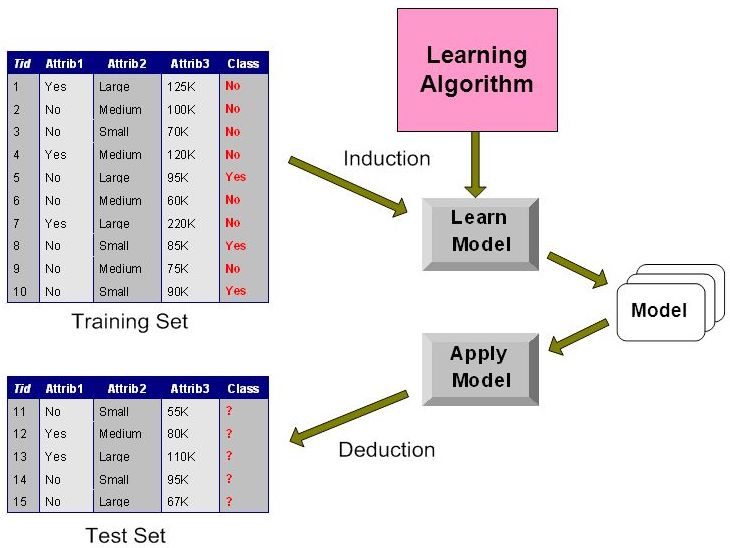
\includegraphics[scale=0.5]{figures/classification.jpg}
    \caption{Typical Classification Task}
\end{figure}

\subsection{Decision Tree}

A tree is built by splitting the source set, constituting the root node of the tree, 
into subsets, which constitute the successor children. 
The splitting is based on a set of splitting rules based on classification features. 
This process is repeated on each derived subset in a recursive manner called recursive partitioning. 
The recursion is completed when the subset at a node has all the same values of the target variable, 
or when splitting no longer adds value to the predictions. 
This process of top-down induction of decision trees is an example of a greedy algorithm, 
and it is by far the most common strategy for learning decision trees from data.

\medskip
Decision trees used in data mining are of two main types:

\begin{itemize}
    \item Classification tree analysis - When the predicted outcome is the class (discrete) to which the data belongs.
    \item Regression tree analysis - When the predicted outcome can be considered a real number.
\end{itemize}

\bigskip
\begin{figure}[H]
    \centering
    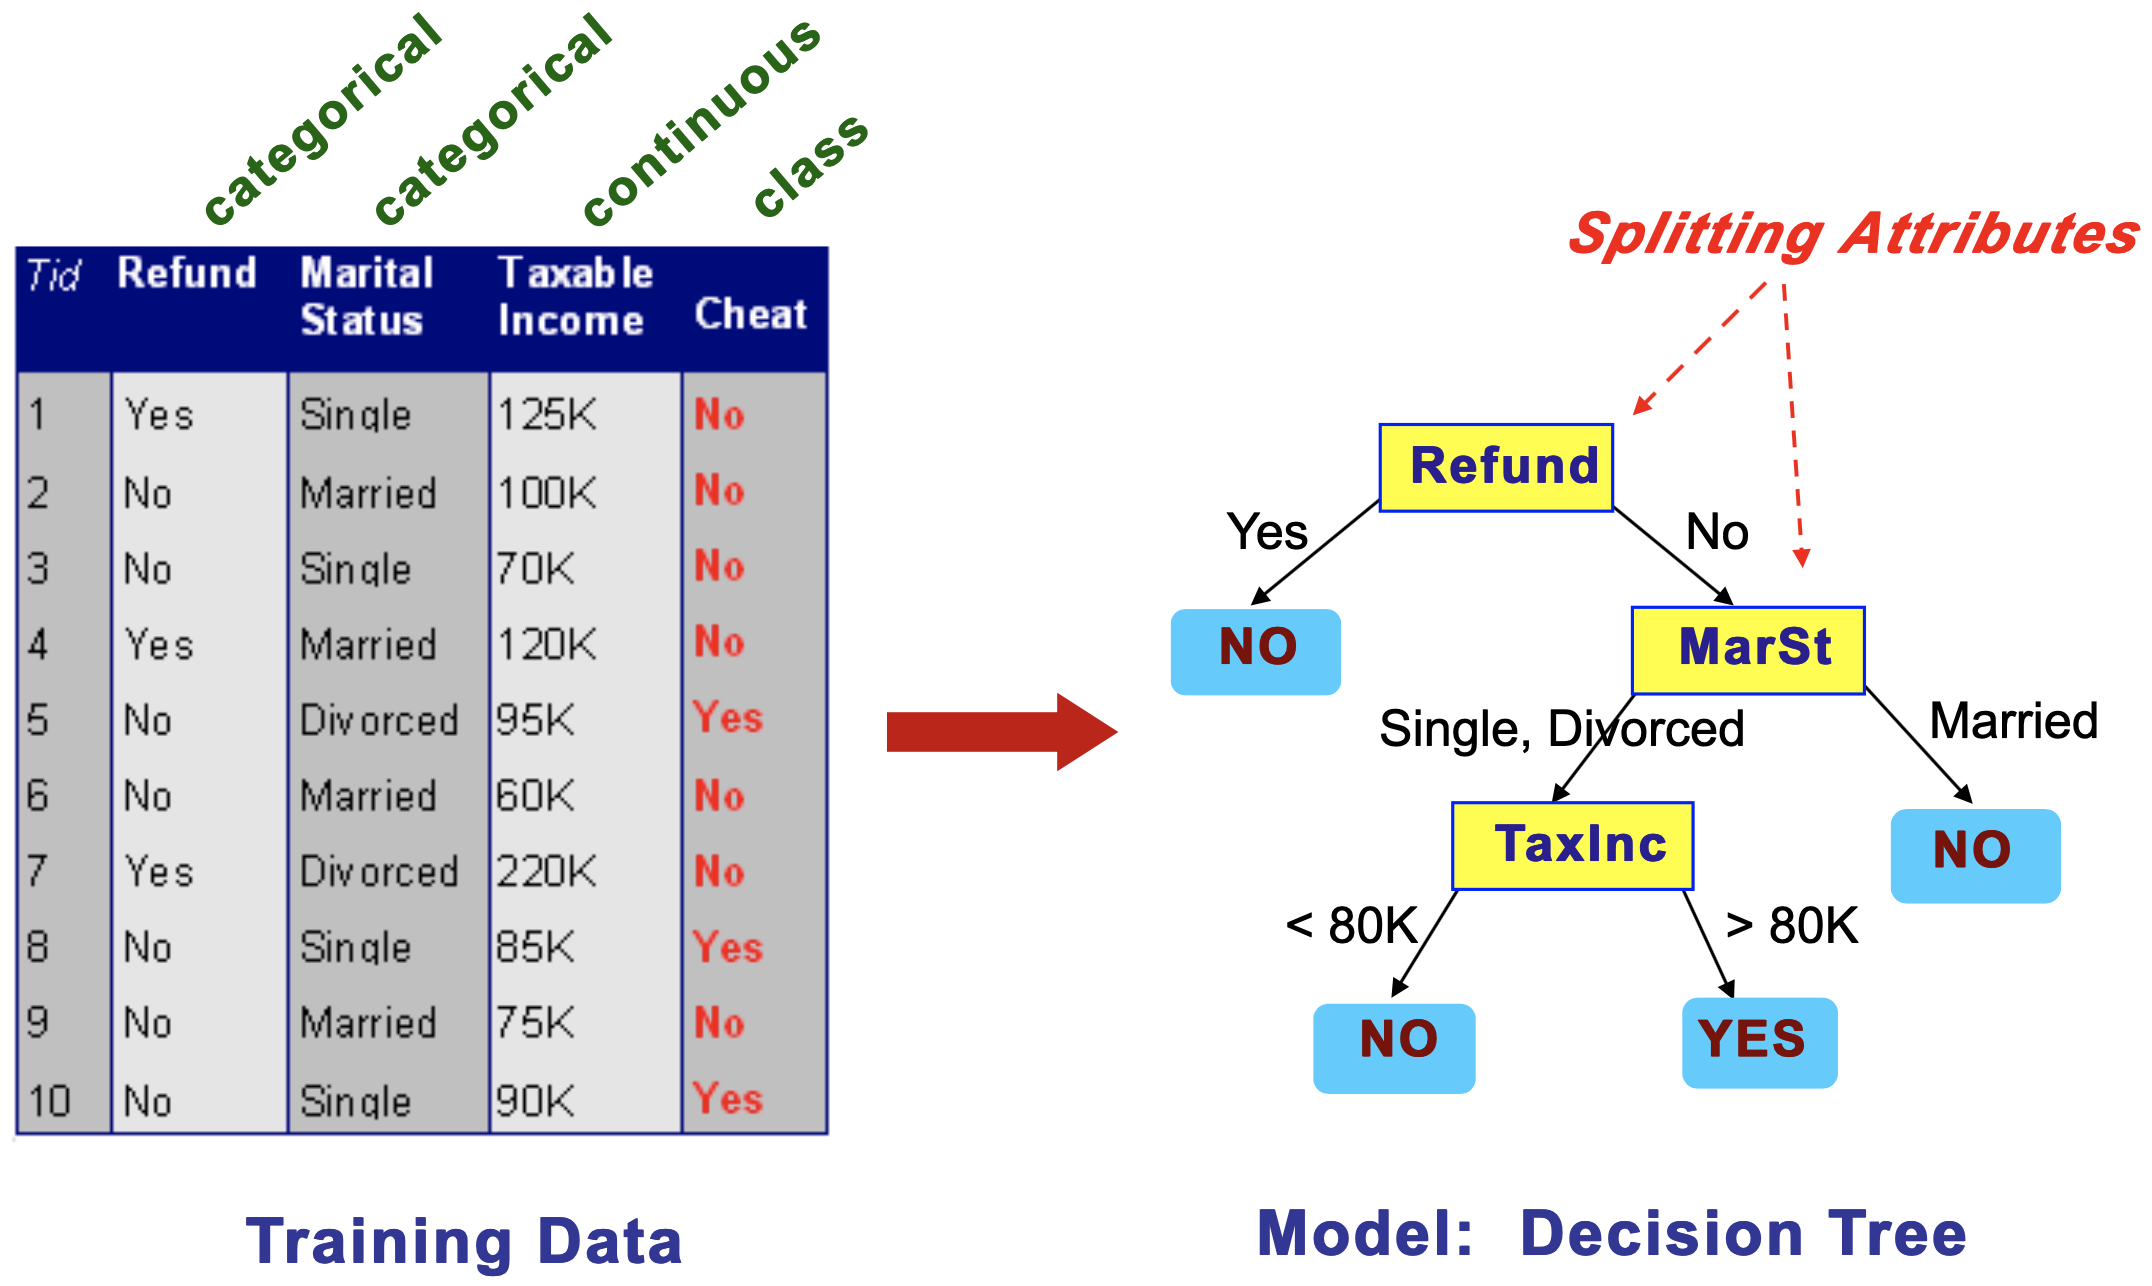
\includegraphics[scale=0.35]{figures/decisiontree.png}
    \caption{Typical Decision Tree}
\end{figure}

\newpage
\section{Hunt's Algorithm}

\begin{itemize}
    \item Let $D_t$ be the set of training records that reach a node $t$.
    \item General procedure:
    \begin{itemize}
        \item If $D_t$ contains records that belong to the same class as $y_t$, then $t$ is a leaf node labeled as $y_t$.
        \begin{itemize}
            \item This is a pure node.
        \end{itemize}
        \item If $D_t$ is an empty set, then $t$ is a leaf node labeled by the default class $y_d$.
        \item If $D_t$ contains records that belong to more than one class, use an attribute test to split the data into smaller subsets. Recursively apply the procedure to each subset.
        \begin{itemize}
            \item This is an impure node.
        \end{itemize}
    \end{itemize}
\end{itemize}

\section{Building Trees}
\subsection{Tree Induction}

The greedy strategy splits the records based on an attribute test that optimizes a certain criterion.

Issues with this approach include:
\begin{itemize}
    \item How to split the records. How should the attribute test condition be specified, and how is the best split determined?
    \item Determining when to stop.
\end{itemize}

\subsubsection{Specifying the Attribute Test Condition}
A proper test condition depends on the attribute type, which can be nominal, ordinal, or continuous.
\medskip

The condition also depends on the number of ways to split. This can be either a two-way split (binary) or a multi-way split. The binary split is often preferred as of the bushiness of the multi-way split. This means that very few records will match the leaf-nodes, and will therefore be overfitted.
\medskip

Ordinal attributes can be split the same way as nominal attributes, with some limitations if the order is to be preserved.
\medskip

For continuous attributes, there are two ways of handling splitting:
\begin{itemize}
    \item Discretization to form an ordinal catergorical attribute.
    \begin{itemize}
        \item Static - discretize once at the beginning.
        \item Dynamic - ranges can be found by equal interval bucketing, equal frequency bucketing, or clustering.
    \end{itemize}
    \item Binary decision.
    \begin{itemize}
        \item Consider all possible splits and find the best cut.
        \item Can be more compute intensive.
    \end{itemize}
\end{itemize}

\subsubsection{Determine Best Split}
When it comes to greedy approaches, nodes with a homogeneous class distribution are preffered.
\bigskip
\begin{figure}[H]
    \centering
    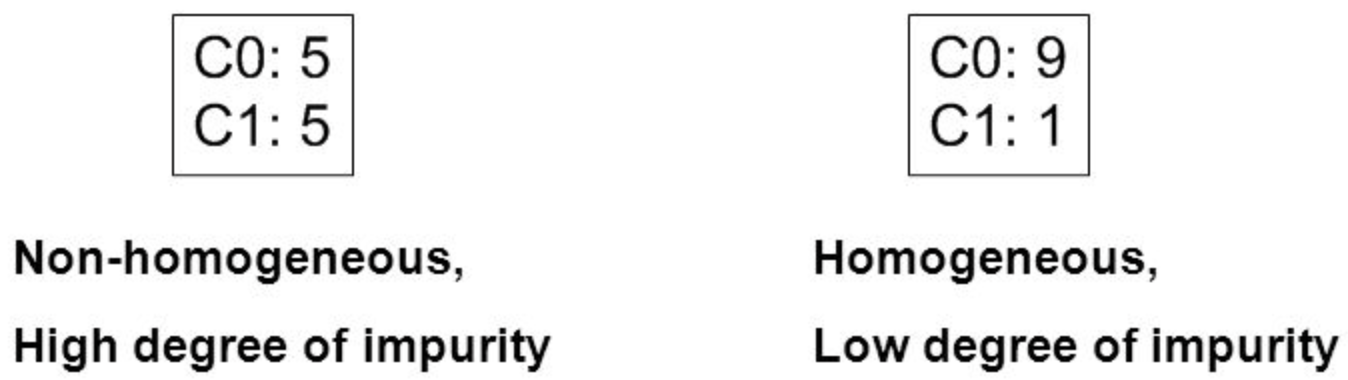
\includegraphics[scale=0.5]{figures/bestsplit.png}
    \caption{Class distributions}
\end{figure}

\section{Measures of Node Impurity}
Finding the best split follows closely to this process:

\begin{enumerate}
    \item Define the set of records as $M0$, where some records belong to class $C0$, while the rest belongs to $C1$.
    \item Define some splitting criterias $A$ and $B$.
    \item Use each criteria to generate new sets of records. The new sets of records now has a different (or equal) distribution of $C0$- and $C1$-records.
    \begin{itemize}
        \item $M1$ and $M2$ from $A$, collected into $M12$
        \item $M3$ and $M4$ from $B$, collected into $M34$
    \end{itemize}
    \item The gain in purity can be measured as such: $Gain = M0 - M12 \text{ vs. } M0 - M34$
    \item The greedy algorithm can then choose the attribute that gives the greatest gain in purity.
\end{enumerate}

\newpage
\subsection{Gini}
The Gini Index measures the degree of probability of a particular variable being wrongly classified when it is randomly chosen.

\begin{theo}[Gini Index]{theo:theo10}
    \label{eq:giniindex}
        \[
            GINI(t) = 1 - \sum_j^{n_c}\left[p(j|t)\right]^2
        \]
        \begin{center}
            Maximum: $(1-\frac{1}{n_c})$ \qquad\qquad Minimum: $0.0$ (pure)
        \end{center}
        Note: $p(j|t)$ is the relative frequency of class $j$ at node $t$.
\end{theo}

Gini can be used when splitting nodes. When a node $p$ is split into $k$ partitions (children), the quality of split follows the theorem:

\begin{theo}[Gini Split]{theo:theo11}
    \label{eq:ginisplit}
        \[
            GINI_{split} = \sum_{i=1}^{k}\frac{n_i}{n}GINI(i)
        \]
        $n_i$ = Number of records at child $i$.

        $n$ = Number of records at node $p$.
\end{theo}

Compute the Gini Index for continuous attributes can often be quite expensive as all values have to be evaluated for splitting.
One process (to be done for each attribute) for finding a good split is as such:

\begin{enumerate}
    \item Sort the attribute on values.
    \item Linearly scans the values, each time choosing the mean of the current value and the next value as the splitting point position and compute the Gini Index.
    \item Choose the split position that has the least Gini Index.
\end{enumerate}

\begin{figure}[H]
    \centering
    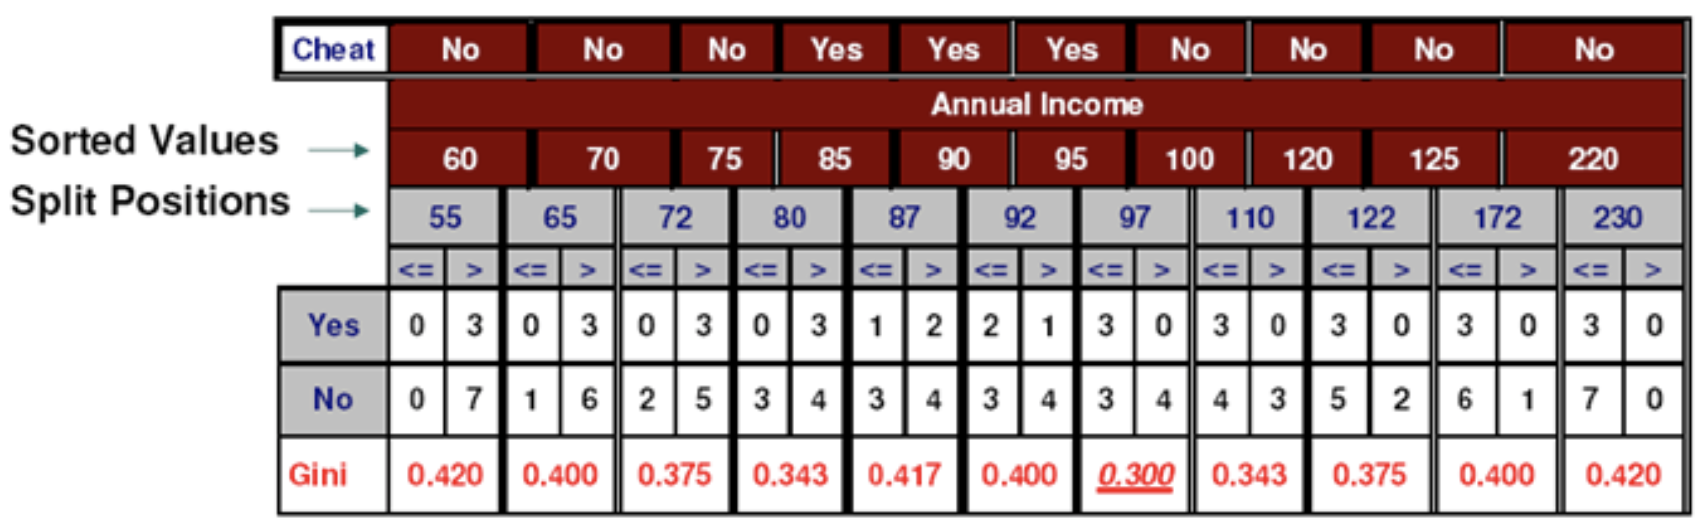
\includegraphics[scale=0.4]{figures/continuousgini.png}
    \caption{Gini Index of Continuous Attributes}
\end{figure}

\subsection{Entropy}
Entropy is a measure of the uncertainty associated with a random variable. Entropy is a splitting criterion based on information gain and measures the homogeneity of a node.


\bigskip
\begin{theo}[Entropy]{theo:theo12}
    \label{eq:entropy}
        \[
           Entropy(t) = -\sum_j^{n_c} p(j|t)\log_2 \text{ } p(j|t)
        \]
        \begin{center}
            Maximum: $(\log_2 \text{ } n_c)$ \qquad\qquad Minimum: $0.0$
        \end{center}
        Note: $p(j|t)$ is the relative frequency of class $j$ at node $t$.
\end{theo}

In the same way Gini can be used to split nodes, so can Entropy:

\bigskip
\begin{theo}[Entropy Split]{theo:theo13}
    \label{eq:entropysplit}
        \[
            GAIN_{split} = Entropy(p) - \left(\sum_{i=1}^k \frac{n_i}{n} Entropy(i)\right)
        \]
        Parent node $p$ is split into $k$ partitions.

        $n_i$ is the number of records in partition $i$
\end{theo}

The gain measures reduction in entropy achieved from the split. Choose the split that achieves the most reduction, that is, maximizes gain.

The disadvantage is that Entropy tends to prefer splits that result in a large number of partitions, each being small but pure (overfitting).

This is fixed by including the number of partitions in the equation.

\bigskip
\begin{theo}[Entropy Split Ratio]{theo:theo14}
    \label{eq:entropysplitratio}
        \[
            GainRation_{split} = \frac{Gain_{split}}{SplitInfo}
        \]
        \[
            SplitInfo = -\sum_{i=1}^k \frac{n_i}{n} \log\frac{n_i}{n}
        \]
        Parent node $p$ is split into $k$ partitions.

        $n_i$ is the number of records in partition $i$
\end{theo}

\subsection{Misclassification error}
The Classification error measures the misclassification error made by a node.

Classification error at node $t$:

\bigskip
\begin{theo}[Classification Error]{theo:theo15}
    \label{eq:classificationerror}
        \[
            Error(t) = 1-\max P(i|t)
        \]
        \begin{center}
            Maximum: $(1-\frac{1}{n_c})$ \qquad\qquad Minimum: $0.0$
        \end{center}
\end{theo}

\subsection{Comparison among Splitting Criterias}

\bigskip
\begin{figure}[H]
    \centering
    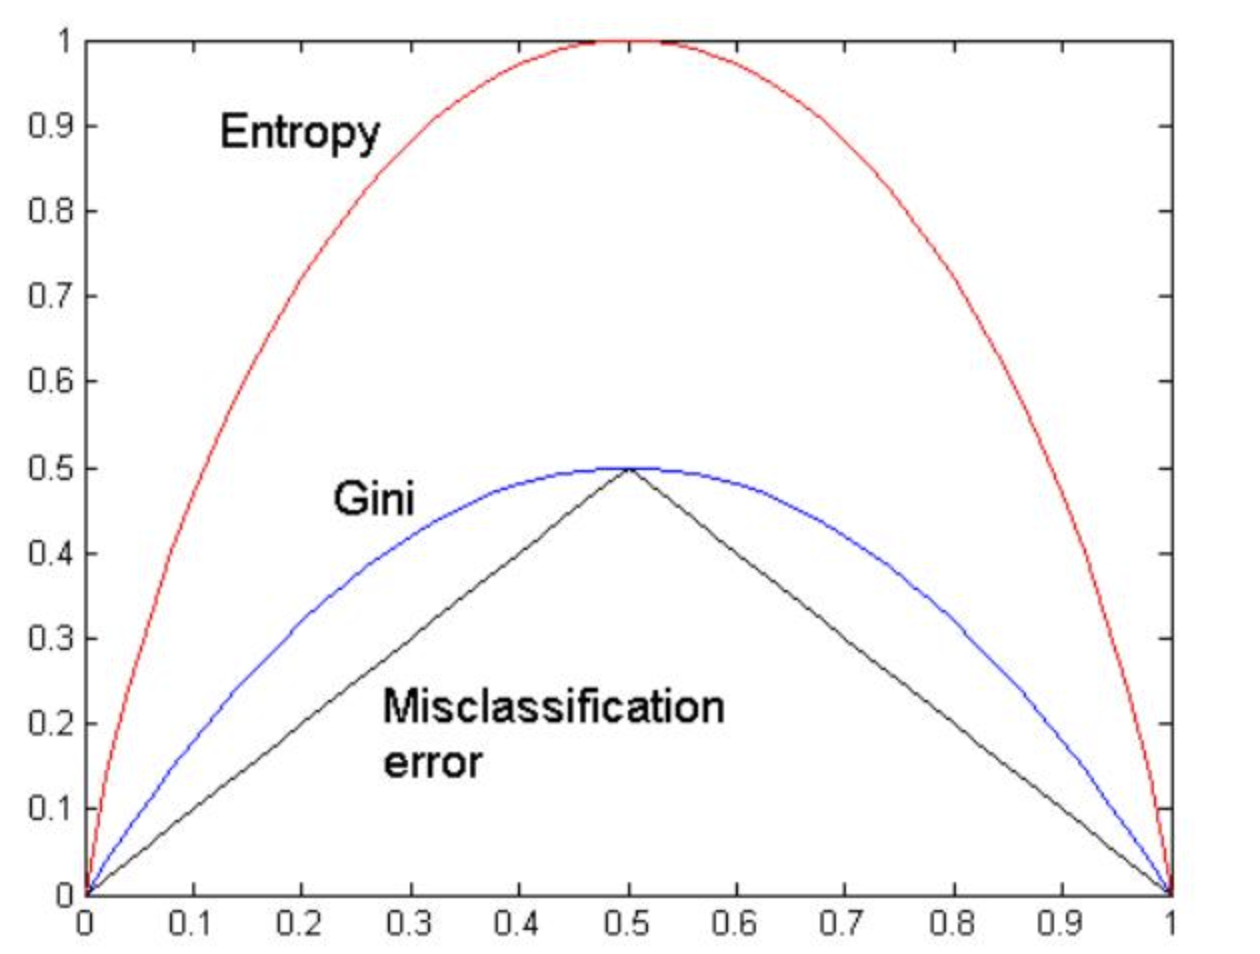
\includegraphics[scale=0.5]{figures/splittingcomparison.png}
    \caption{Splitting Criterias for a two-class problem}
\end{figure}

\section{Stopping Criteria for Tree Induction}
\begin{itemize}
    \item Stop expanding a node when all the records belong to the same class.
    \item Stop expanding a node when all the records have similar attribute values.
    \item Early termination (probably for limiting tree depth).
\end{itemize}

\section{Advantages of Decision Tree based Classification}
\begin{itemize}
    \item Inexpensive to construct.
    \item Extremely fast at classifying unknown records.
    \item Easy to interpret for small-sized trees.
    \item Accuracy is comparable to other classification techniques for many simple data sets.
\end{itemize}

\section{Classification Issues}
\subsection{Underfitting and Overfitting}
\begin{itemize}
    \item Underfitting: When a model cannot capture the underlying trend of the data. Intuitively, underfitting occurs when the model or the algorithm does not fit the data well enough. Specifically, underfitting occurs if the model or algorithm shows low variance but high bias. Underfitting is often a result of an excessively simple model. Overfitting can also arise from insufficient data points.
    \item Overfitting: When a model captures the noise of the data. Intuitively, overfitting occurs when the model or the algorithm fits the data too well. Specifically, overfitting occurs if the model or algorithm shows low bias but high variance. Overfitting is often a result of an excessively complicated model, and it can be prevented by fitting multiple models and using validation or cross-validation to compare their predictive accuracies on test data.
\end{itemize}
\bigskip
\begin{figure}[H]
    \centering
    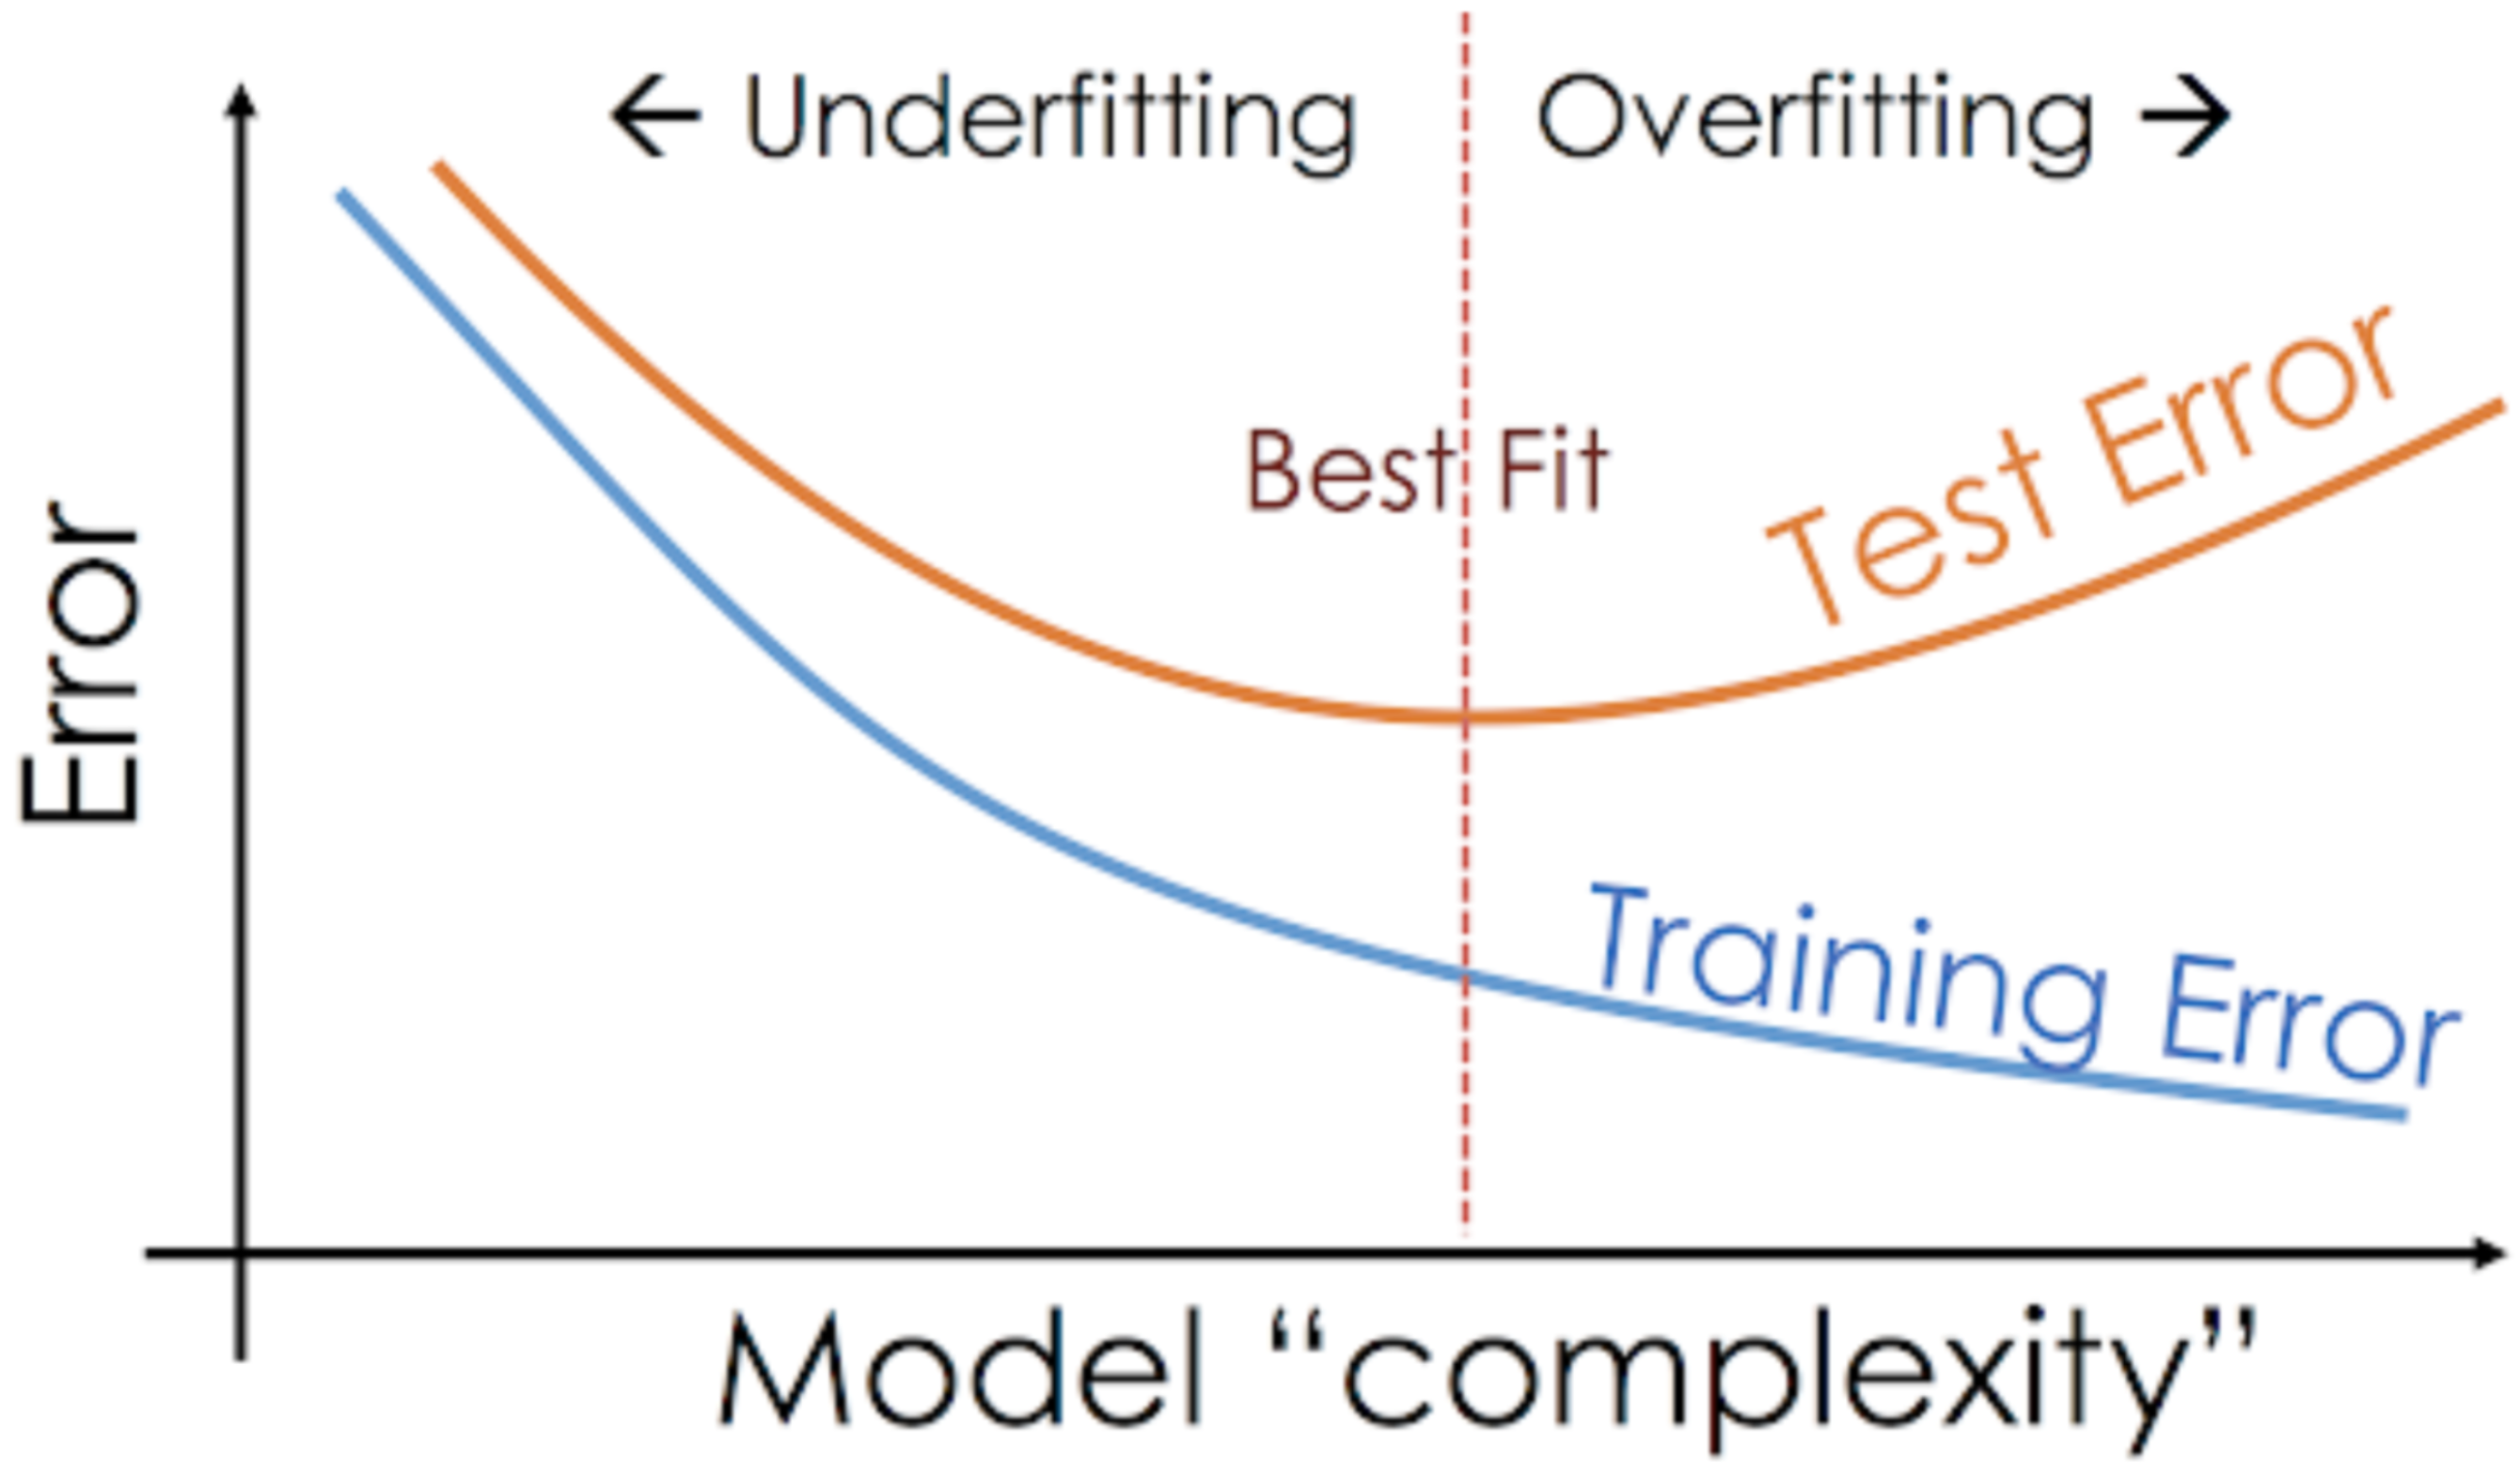
\includegraphics[scale=0.25]{figures/overunderfitting.png}
    \caption{Overfitting and underfitting}
\end{figure}

\subsection{Address Overfitting}
\subsubsection{Decision Tree Pruning}
Pre-Pruning (Early Stopping Rule):
\begin{itemize}
    \item Stop the algorithm before it becomes a fully-grown tree.
    \begin{itemize}
        \item Stop if all instances belong to the same class.
        \item Stop if all the attribute values are the same.
        \item Stop if the number of records in a node are lower than the user-specified threshold.
        \item Stop if splitting a node does not improve the impurity meassure.
    \end{itemize}
\end{itemize}

Post-Pruning:
\begin{enumerate}
    \item Grow decision tree to its entirety.
    \item Trim the nodes of the decision tree in a bottom-up fashion.
    \item If generalization error improves after trimming, replace sub-tree by a leaf node.
    \item The class label of a leaf node is determined from the majority class of instances in the sub-tree.
\end{enumerate}

\subsubsection{Occam's Razor}
\begin{itemize}
    \item Given two models of similar generalization errors, one should prefer the simpler model over the more complex model.
    \item For complex models, there is a greater chance that it was fitted accidentally by the error in data.
    \item Therefore, one should include model complexity when evaluating a model.
\end{itemize}

\subsection{Generalization Errors}
Generalization error is a measure of how accurately a model can predict outcome values for previously unseen data.
The measure is calculated from the ratio of misclassifications that can occur when choosing the majority class for all records in the node.

\begin{itemize}
    \item Training errors: Error on training ($\sum_{t=1}^n e(t)$)
    \item Generalization errors: Error on validation ($\sum_{t=1}^n e'(t)$)
\end{itemize}

Methods for estimating generalization errors:
\begin{itemize}
    \item Optimistic approach: $e'(t) = e(t)$
    \item Pessimistic approach:
    \begin{itemize}
        \item For leaf each leaf node, $e'(t_i) = e(t_i)+\frac{1}{2}$
        \item Total error: $e'(T) = e(T) + N\frac{1}{2}$ ($N$ = number of leaf nodes)
    \end{itemize}
    \item Reduced error pruning (REP)
    \begin{itemize}
        \item Uses validation data set to estimate generalization error.
    \end{itemize}
\end{itemize}

\subsection{Handling Missing Attribute Values}
Missing attribute values affect the decision tree in three major ways:
\begin{itemize}
    \item How impurity measures are computed.
    \item How to distribute instance with missing value to child nodes.
    \item How a test instance with missing value is classified.
\end{itemize}

\subsubsection{Computing Impurity Measure (Impurity Gain)}
One way of computing the information gain is as normal, without including the instances with the missing attribute.
This means that the entropy-computation for the parent is as normal, but for the children, instances with the missing attributes should be omitted, but included in the denominator. Finally, the gain is computed as normal but is multiplied by the fraction of "valid" records.

\subsubsection{Distributing Instances}
\begin{figure}[H]
    \centering
    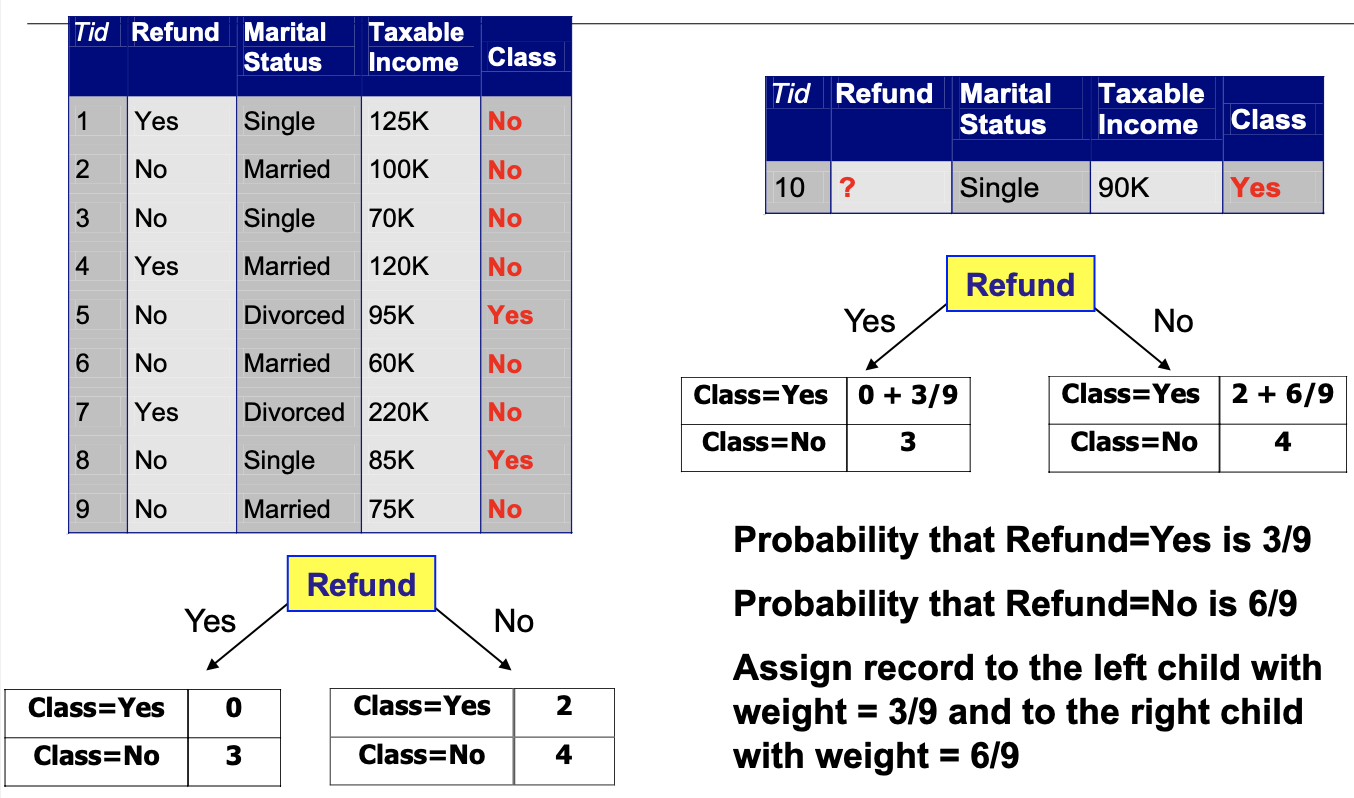
\includegraphics[scale=0.5]{figures/distributeinstances.png}
    \caption{Distributing Instances}
\end{figure}
The figure explains that since the instance with the unknown attribute corresponds to the class yes, it is distributed on both nodes, affecting the yes-class in each node.
The distribution ratio is based on the number of instances of the same class, divided by the total number of instances.

\subsubsection{Classify Instances}
To classify an instance with an unknown class, as well as having the current attribute unknown, can be done by understanding what option is more likely.
If most of the instances are of attribute 1 the instance with the unknown attribute is assumed to also have attribute 1 and follows the tree accordingly.

\subsection{Other Issues}
\subsubsection{Data Fragmentation}
\begin{itemize}
    \item The number of instances gets smaller as you traverse down the tree.
    \item Number of instances at the leaf node could be too small to make any statistically significant decision.
\end{itemize}

\subsubsection{Search Strategy}
\begin{itemize}
    \item Finding an optimal decision tree is NP-hard (exponentially).
    \item The algorithm presented so far uses a greedy, top-down, recursive partitioning strategy to induce a reasonable solution.
    \item Could use bottom-up or bi-directional algorithms.
\end{itemize}

\subsubsection{Expressiveness}
Decision trees provide expressive representation for learning discrete-valued functions, but they do not generalize well to certain types of boolean functions like parity functions.

Also, decision trees are not expressive enough for modeling continuous variables.

\subsubsection{Decision Boundary}
The borderline between two neighboring regions of different classes is known as a decision boundary.

A decision boundary is parallel to the axes because the test conditions only involve a single attribute at a time.

This could be fixed with oblique decision trees, but includes more expressive representation and can be computationally expensive.

\subsubsection{Tree Replication}
The same subtree appears in multiple branches.



\chapter{Model Evaluation}
\section{Metrics for Performance Evaluation}
Metrics for performance evaluation focuses on the predictive capability of a model, that is, how well a model can predict the class of the test data, and evaluate the performance of the training-data.
This focus is instead of focusing on how fast it takes to classify or build models, scalability, etc.

\subsection{Confusion Matrix}
This can be done through a confusion matrix:

\bigskip
\begin{figure}[H]
    \centering
    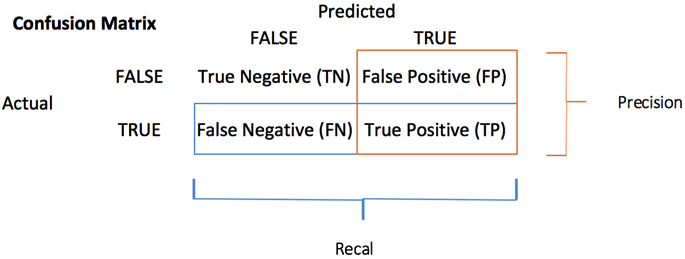
\includegraphics[scale=0.5]{figures/confusionmatrix.png}
    \caption{Confusion Matrix}
\end{figure}

One of the most common and widely-used metric for evaluating the performance is accuracy:

\begin{theo}[]{theo:theo500}
    \label{eq:accuracy}
        \[
            Accuracy = \frac{TP + TN}{TP + TN + FP + FN}
        \]
\end{theo}

The accuracy metric has some limitations, among those are the ability to evaluate two-class problems where almost all instances are of class 0, while only a few are of class 1.
The accuracy metric will result in $99.9\%$ accuracy, which is misleading if the model predicts all instances to belong to class 0.

\subsection{Cost Matrix}

One way of solving the issue is to use a cost matrix instead:

\bigskip
\begin{figure}[H]
    \centering
    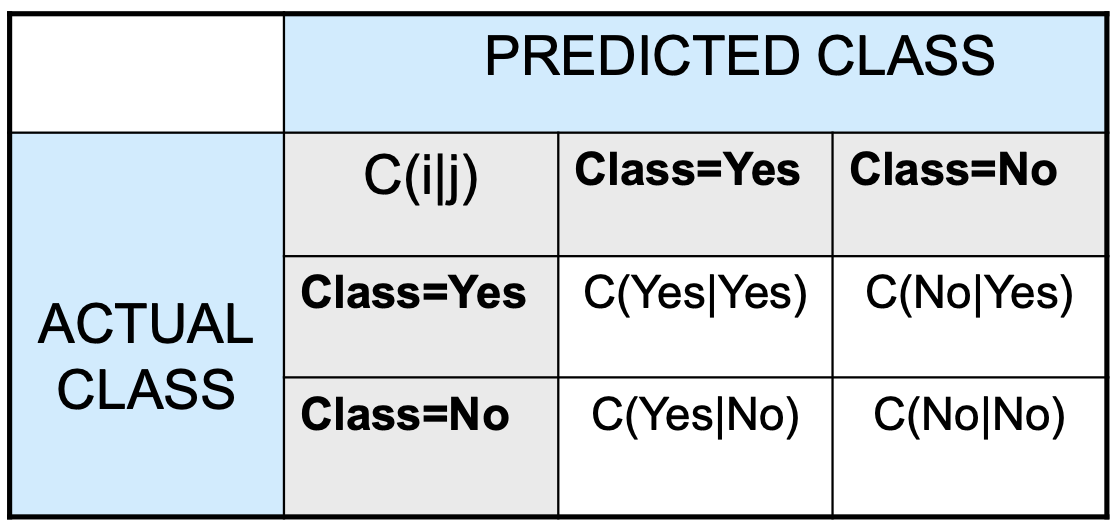
\includegraphics[scale=0.5]{figures/costmatrix.png}
    \caption{Cost Matrix}
\end{figure}

Here, $C(i|j)$ is the cost of misclassifying class $j$ as class $i$. The cost equals the weighted sum of all predictions.

\bigskip

If true positives and true negatives are equally weighted, as well as the fasle positives and the false negatives, the accuracy is proportional to the cost.
This results in the following equation:

\begin{equation}
    Cost = N[q-(q-p)*Accuracy]
\end{equation}
\begin{center}
    Where $N = TP + TN + FP + FN$, $q = FP$, and $p = TP$.
\end{center}


\subsection{Cost-Sensitive Measures}
Some cost-sensitive measures that are preferred over accuracy:

\begin{equation}
    Precision(p) = \frac{TP}{TP+FP}
\end{equation}

\begin{equation}
    Recall(r) = \frac{TP}{TP+FN}
\end{equation}

\begin{equation}
    F-measure(F) = \frac{2TP}{2TP+FP+FN}
\end{equation}

\begin{itemize}
    \item Precision is biased towards $TP$ and $FP$
    \item Recall is biased towards $TP$ and $FN$
    \item F-measure is biased towards all except $TN$
\end{itemize}

\begin{equation}
    Weighted_Accuracy = \frac{\omega_1 TP + \omega_4 TN}{\omega_1 TP + \omega_2 FN + \omega_3 FP + \omega_2 TN}
\end{equation}

\section{Methods for Performance Evaluation}
Methods on how to obtain a reliable estimate of performance.

The performance of a model may depend on other factors besides the learning algorithm:
\begin{itemize}
    \item Class distribution.
    \item Cost of misclassification.
    \item Size of training and test sets.
\end{itemize}

\subsection{Learning Curve}
Learning curves show how accuracy changes with varying sample sizes.

Learning curves require a sampling schedule:
\begin{itemize}
    \item Arithmetic sampling. (Linear)
    \item Geometric sampling. (Exponential)
\end{itemize}

\bigskip
\begin{figure}[H]
    \centering
    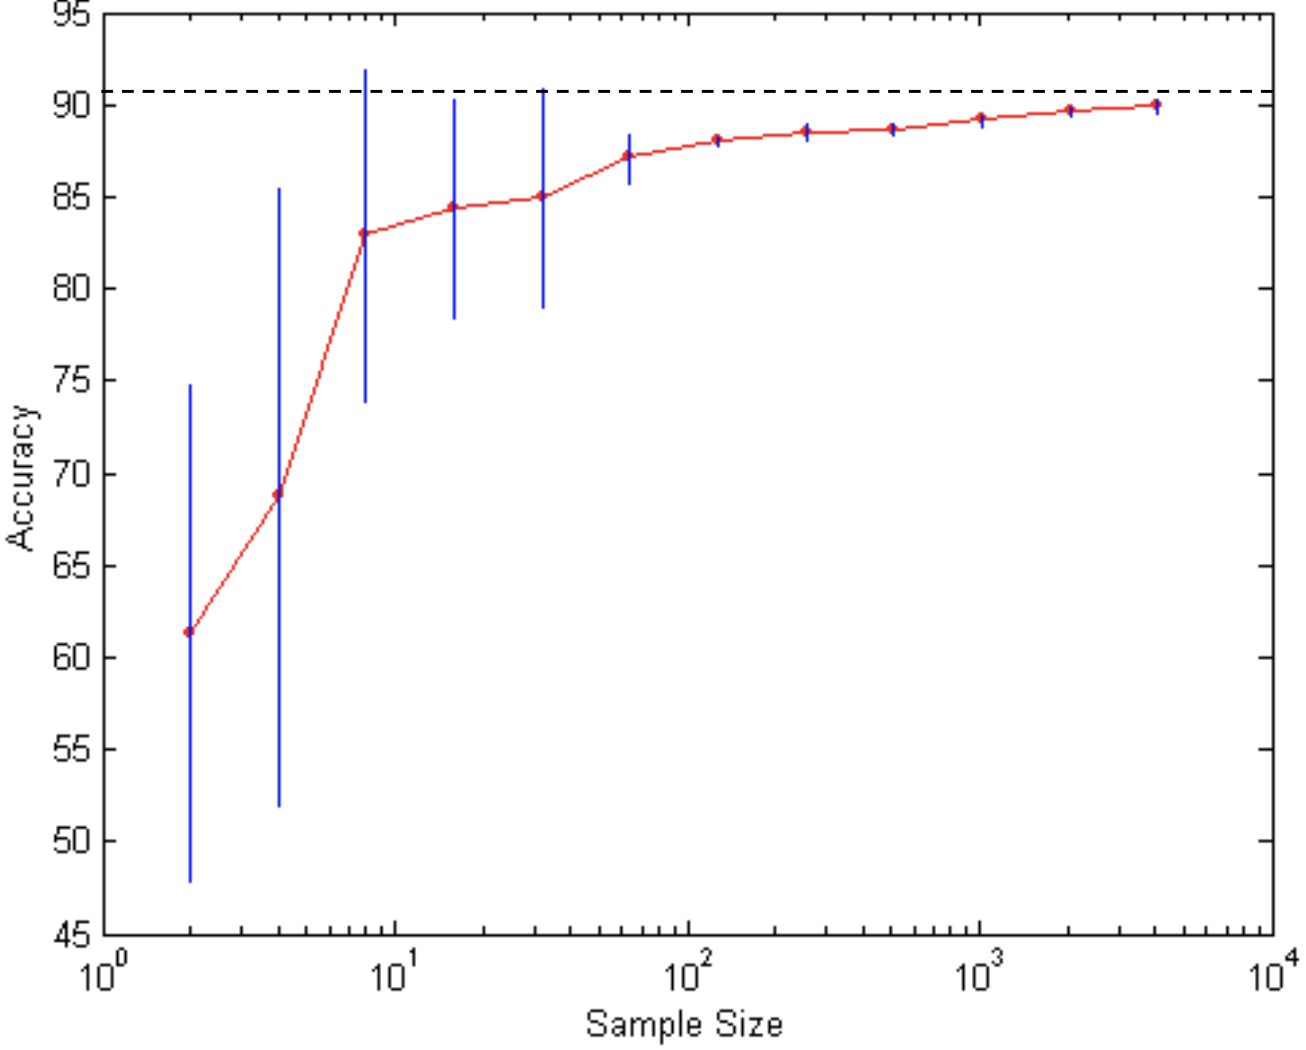
\includegraphics[scale=0.5]{figures/learningcurve.png}
    \caption{A Learning Curve}
\end{figure}

The effects of small sample sizes includes:
\begin{itemize}
    \item Bias in the estimate (Underfitting)
    \item Variance of estimate (Overfitting)
\end{itemize}

\subsection{Other Methods of Estimation}
\begin{itemize}
    \item Holdout
    \begin{itemize}
        \item Reserve $80\%$ for training and $20\%$ for testing.
    \end{itemize}
    \item Random subsampling
    \begin{itemize}
        \item Repeated holdouts
    \end{itemize}
    \item Cross validation (popular)
    \begin{itemize}
        \item Partition data into $k$ disjoint subsets.
        \item $k$-fold: Train on $k-1$ partitions, test on the remaining one.
        \item Leave-one-out: $k=n$
    \end{itemize}
    \item Stratified sampling
    \begin{itemize}
        \item Oversampling
        \item Undersampling
    \end{itemize}
    \item Bootstrap
    \begin{itemize}
        \item Sampling with replacement
    \end{itemize}
\end{itemize}

\newpage
\section{Methods for Model Comparison}
Methods for model comparison explains how to compare the relative performance among competing models.

\subsection{Receiver Operating Characteristic (ROC)}
ROC was developed in the 1950s to characterize the trade-off between true positives and false positives.

A ROC curve plots $TP$ on the $y$-axis against $FP$ on the $x$-axis, where the performance of each classifier is represented as a point on the ROC curve.
The point changes based on the threshold of the algorithm, the sample distribution, and/or the cost matrix.

\bigskip
\begin{figure}[H]
    \centering
    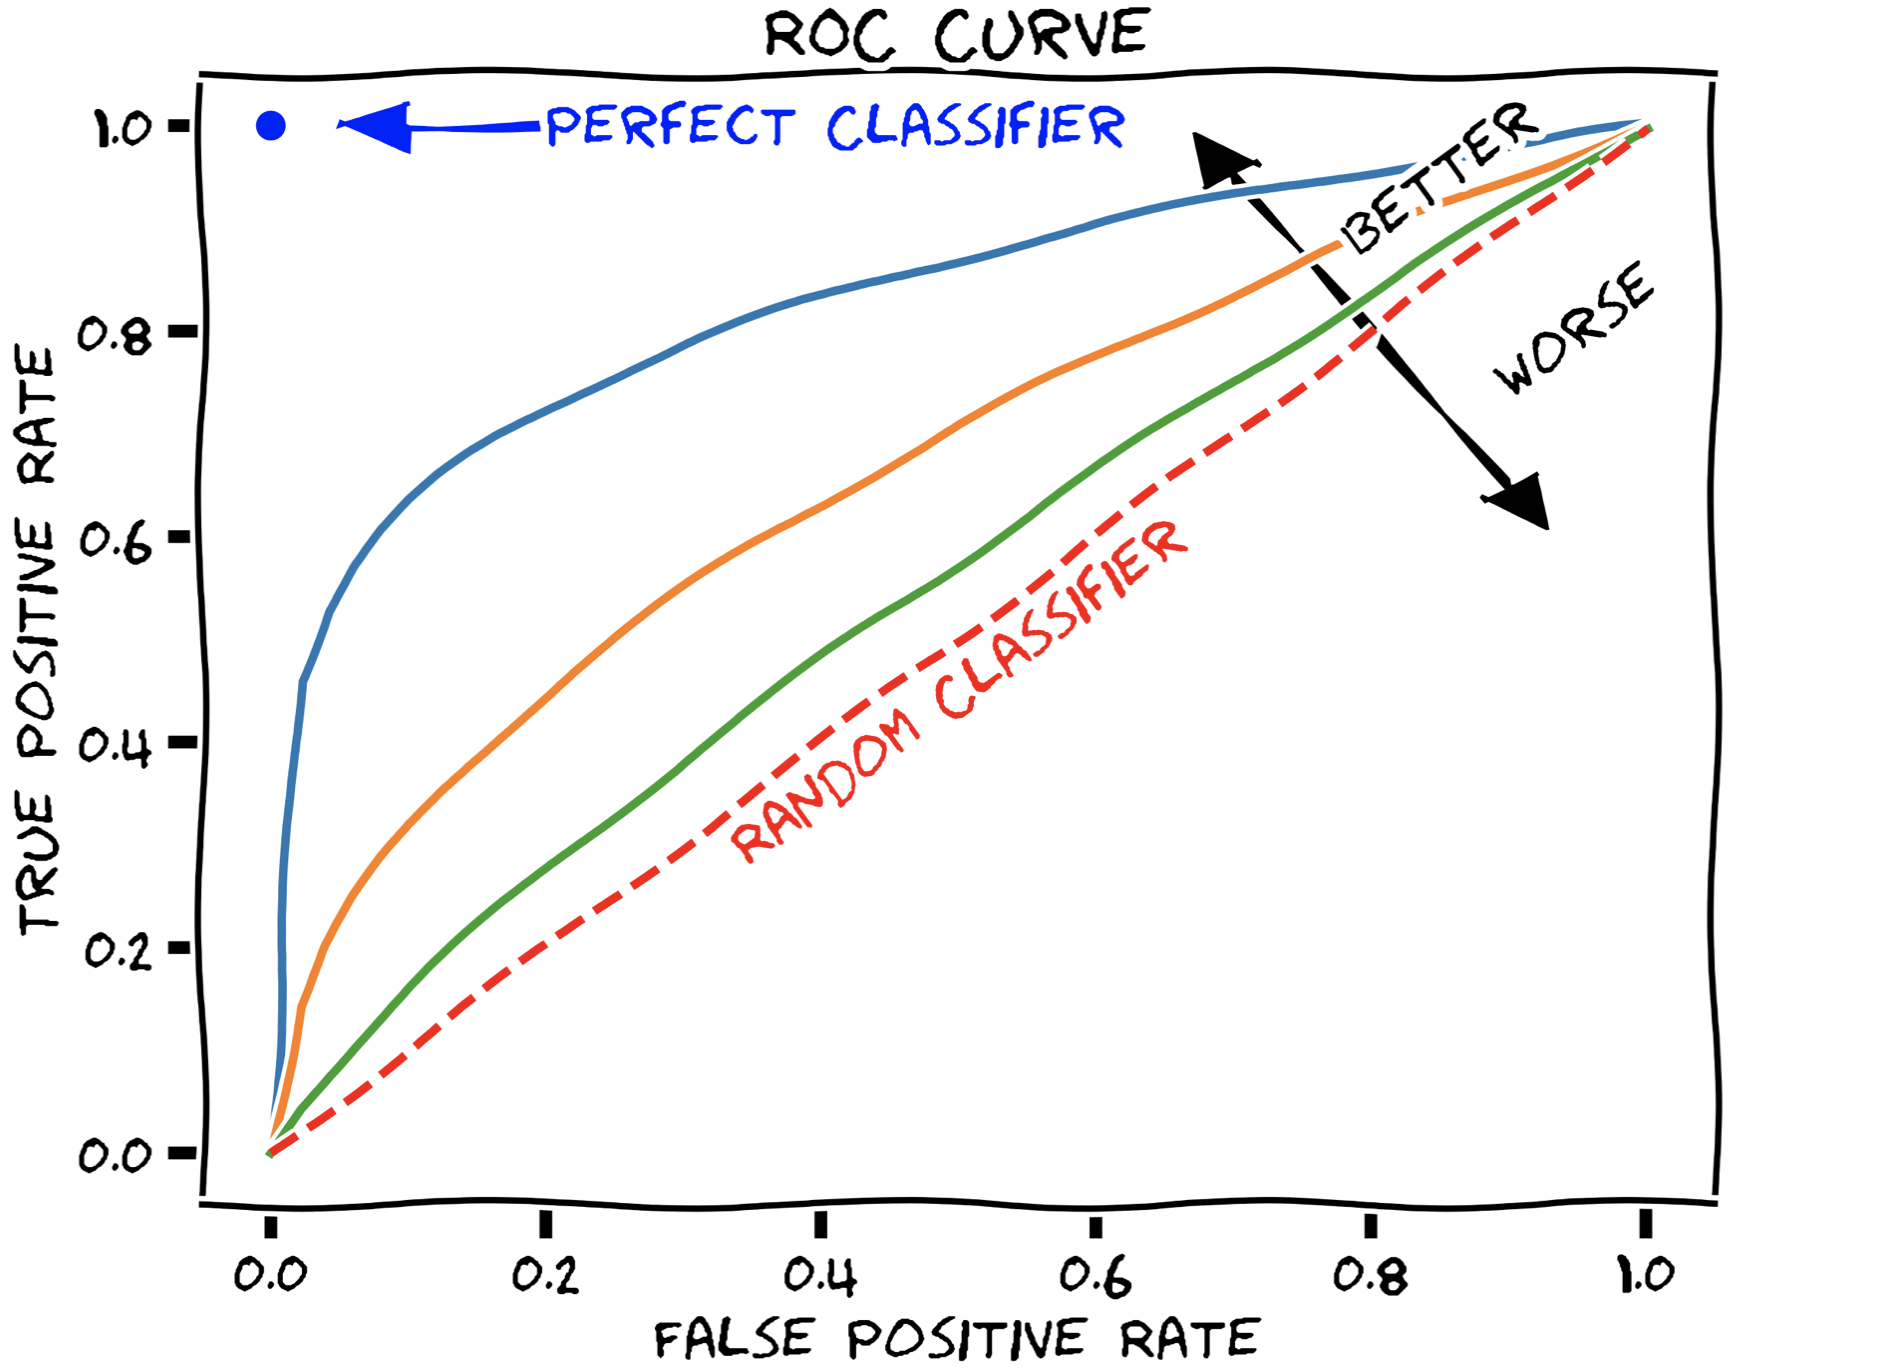
\includegraphics[scale=0.25]{figures/roccurve.png}
    \caption{ROC Curve}
\end{figure}

In some cases when comparing the ROC curve for different models, no models consistently outperform the others. Evaluating such models can be based on the area under the ROC curve (AUC), or which model fits better to the desired outcome.

\subsubsection{Constructing a ROC curve}
\begin{enumerate}
    \item Use a classifier that produces posterior probability for each test instance $P(+|A)$.
    \item Sor the instances according to $P(+|A)$ in decending order.
    \item Apply threshold at each unique value of $P(+|A)$.
    \item Count the number of $TP$, $FP$, $TN$ and $FN$ at each treshold.
\end{enumerate}
\begin{itemize}
    \item $TPR = \frac{TP}{TP+FN}$
    \item $FPR = \frac{FP}{FP+TN}$
\end{itemize}


\chapter{Regression Trees and Ensemble methods}
\section{Regression Trees}
In a decision tree, there is typically a data set with $N$ features ($X_1, X_2, \cdots, X_N$). Each of the features has a domain, with the domain type being dependent on the type of data the feature contains (categorical or numerical).
The output variable $Y$ will have a domain $D_y$.
\begin{itemize}
    \item Categorical - Classification
    \item Numerical - Regression
\end{itemize}

\subsection{Constructing a Regression Tree}

We have already explored the classification algorithm of decisiont trees and how
entropy, gini and information gain is used to calculate node impurity which is
used to determine the splits. But what do we use when the dependent variable $Y$
is a continious / numerical value? Most litterature use two metrics for 
regression trees are  \textit{Least Squares} and the other 
\textit{Least Absolute deviations}. \cite{loh2011classification} 
In both cases the spread in the nodes is used as a metric for 
\textit{information}, in the same way as entropy. The split that has the least
variance in it's child nodes compared to the parent is the split that contains 
the most information.

\begin{enumerate}
    \item Find a split $(X_i, v)$ that creates two child nodes $D_L$ and $D_R$ from the parent node $D$. The split should maximize the weighted sum of the variances.
    \begin{itemize}
        \item For ordered domains, sort $X_i$ and consider a split between each pair of adjacent values.
        \item For categorical $X_i$ find the best split based on subsets (Breiman's algorithm).
    \end{itemize}
\end{enumerate}

\begin{equation}
    \text{Weighted Variance} = \abs{D}*Var(D) - \left(\abs{D_L}*Var(D_L) + \abs{D_R}*Var(D_R)\right)
\end{equation}

\begin{equation}
    \text{Var}(D) = \frac{1}{n}\sum_{i=1}^{\abs{D}}(y_i-\overline{y})^2
\end{equation}

\subsubsection{Stopping a Tree}
\begin{itemize}
    \item When the leaf is pure, i.e. $Var(D) < \epsilon$
    \item When the number of instances in the leaf $(\abs{D})$ is too small.
\end{itemize}

\subsubsection{Predictor}
\begin{itemize}
    \item Regression - Average value of $y_i$ of the instances in the leaf.
    \item Classification - Choose the most common $y_i$ in the leaf.
\end{itemize}

\section{Ensemble Methods}
In addition to using pruning to construct more generalised trees. Two other
methods exist to generalise models. These are ensemble and resample methods.
Ensemble methods construct a set of classifiers from a given training data.
The classification is done by predicting class values from previously unseen 
records by aggregating predictions made by multiple classifiers.

\bigskip
The general idea of ensemble methods is to have the original training data and then:
\begin{enumerate}
    \item Create multiple data sets from the training data (resampling).
    \item Build multiple classifiers corresponding to the data sets.
    \item Combine the predictions of the classifiers.
\end{enumerate}

Ensemble methods work the sum of the error rate of multiple independent classifiers are lower than the error rate itself.
The following equation calculates the probability that the ensemble classifier makes a wrong prediction, having $\epsilon$ as the error rate.

\begin{equation}
    \sum_{i=N/2(+1)}^N \genfrac(){0pt}{2}{N}{i} \epsilon^i(1-\epsilon)^{N-i}
\end{equation}

\section{Manipulating the Training set}
\subsubsection{Bagging}
Bagging is sampling with replacement (bootstrapping).

\begin{enumerate}
    \item Let $k$ be the number of bootstrap samples.
    \item \texttt{for $i$ in range($k$):}
    \begin{enumerate}
        \item Create a bootstrap sample of size $N$, $D_i$.
        \item Train a base classifier $C_i$ on the bootstrap sample $D_i$.
    \end{enumerate}
    $C^{*}(x) = argmax\left(\sum_i \delta\left(C_i(x)=y\right)\right)$
\end{enumerate}

$\delta = 1$ if the argument is true and $0$ otherwise (the majority class is chosen).

Bagging can also increase the complexity of simple classifiers such as decision stumps.

\newpage
\subsubsection{Boosting}
Boosting is an iterative procedure to adaptively change the distribution of training data by focusing more on previously misclassified records.
Initially, all $N$ records are assigned equal weights.

Unlike bagging, the weights of the records may change at the end of each boosting round.

\begin{itemize}
    \item Records that are wrongly classified will have their weights increased.
    \item Records that are classified correctly will have their weights decreased.
\end{itemize}

One way of boosting is to use the AdaBoost algorithm:

\begin{figure}[H]
    \centering
    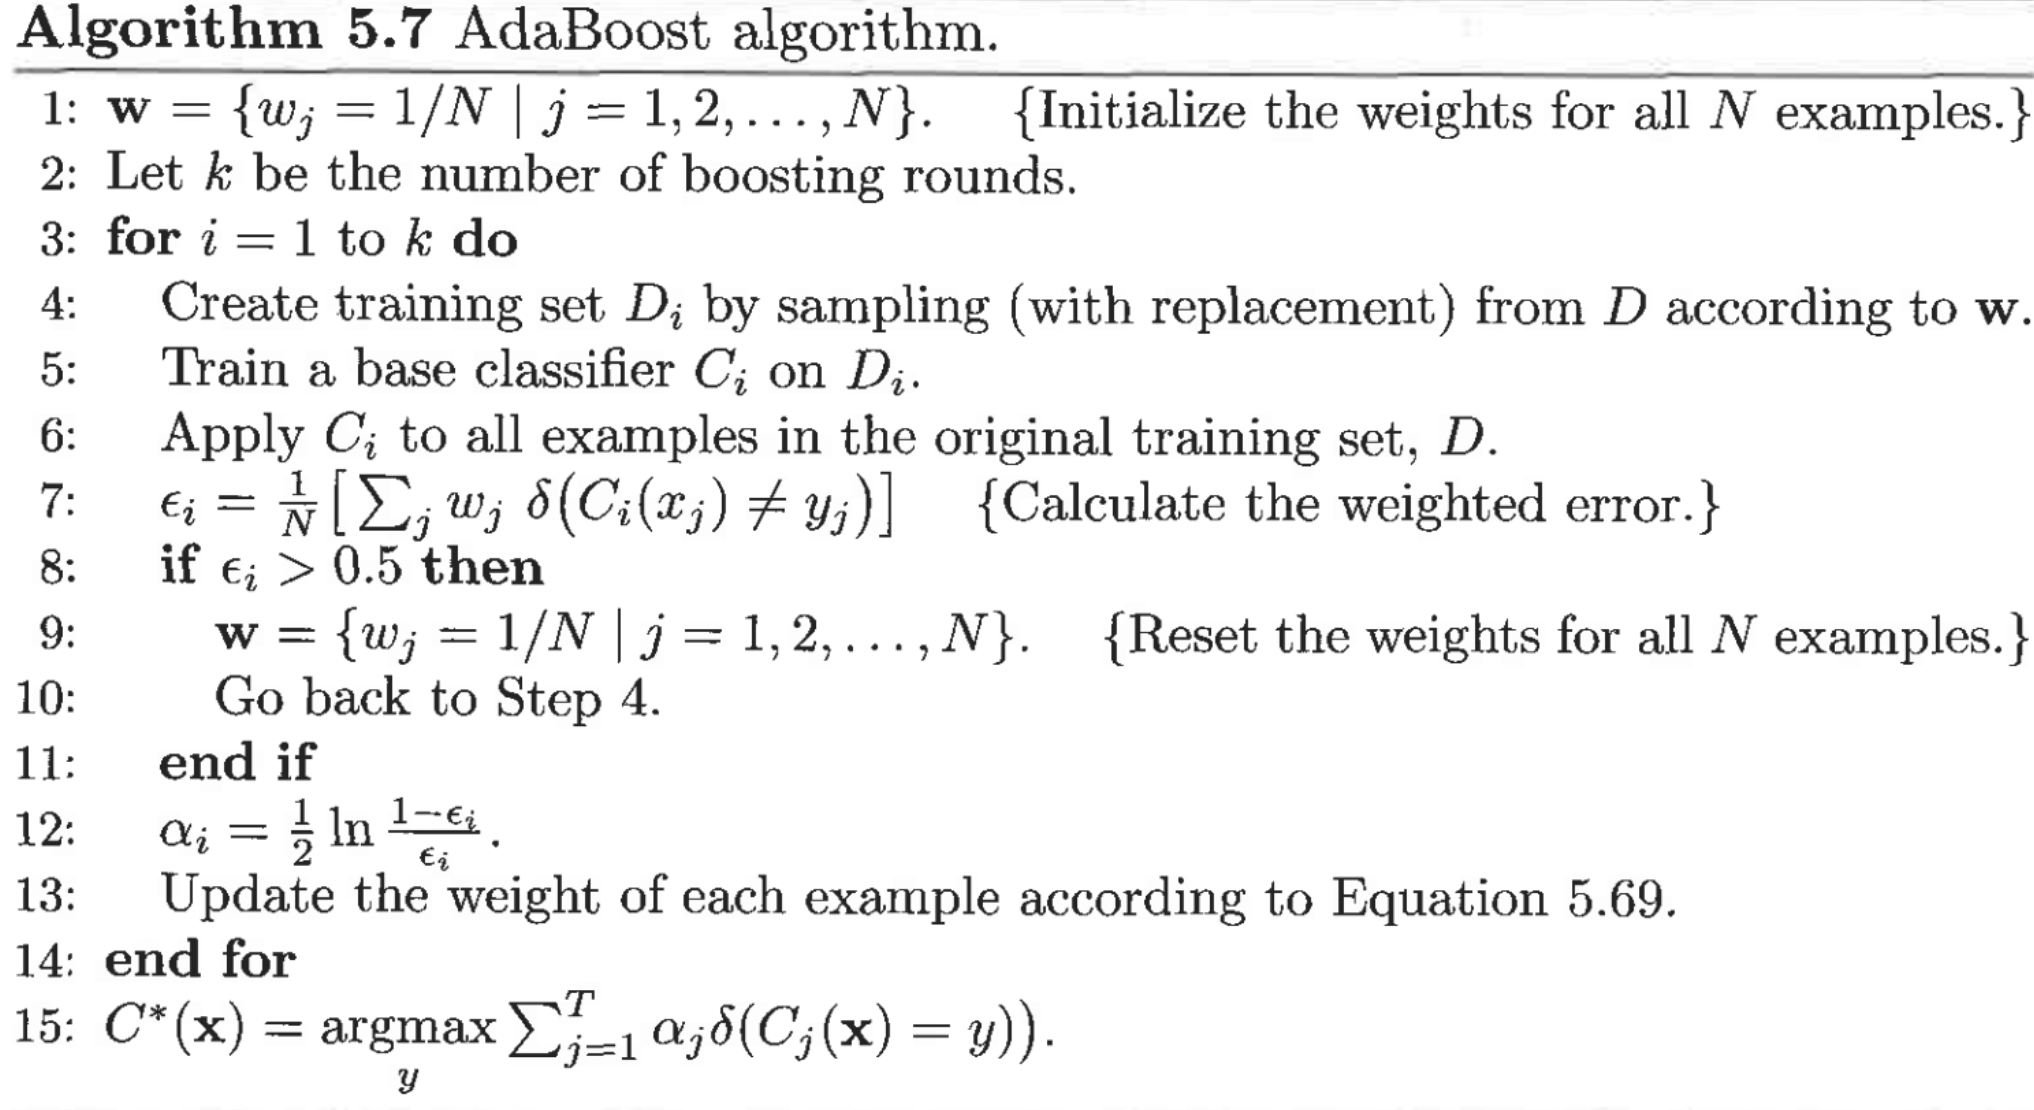
\includegraphics[scale=0.3]{figures/adaboost.png}
    \caption{AdaBoost Algorithm}
\end{figure}

\newpage
\section{Manipulating the Features}
\subsubsection{Random Forest}
A random forest is a class of ensemble methods specifically designed for decision tree classifiers.
It combines the predictions made by multiple decision trees where each tree is generated based on the values of an independent sample set.
The samples are generated from a fixed probability distribution.

\bigskip
As in bagging, we build decision trees on bootstrapped training samples.
Each time a split in a tree is considered, a random sample of $F$ features is chosen as split candidates from the full set of $m$ features.

(If $F=m$, we have bagging)

\bigskip
A random forest algorithm can look like this:
\begin{itemize}
    \item \texttt{for $i$ in range($B$):}
\end{itemize}
\begin{enumerate}
    \item Draw a bootstrap sample $D^{*}$ of size $N$ from the training data.
    \begin{enumerate}
        \item Grow a random forest tree to the bootstrapped data.
        \begin{enumerate}
            \item Select $\bm{F}$ features at random from the $m$ variables.
            \item Pick the best variable/split point among the $\bm{F}$s.
            \item Split the node into two child nodes.
        \end{enumerate}
    \end{enumerate}
\end{enumerate}
\begin{itemize}
    \item Output the ensemble of trees.
\end{itemize}

Prediction at a new point $x$ can be done:
\begin{itemize}
    \item For regression - Average of the results.
    \item For classification - Majority vote.
\end{itemize}

\subsubsection{Random Forest Recommendations}
\begin{itemize}
    \item For classification, the default value for $F$ is $\sqrt{m}$ and the minimum node size is one.
    \item For regression, the default value for $F$ is $\frac{m}{3}$ and the minimum node size is five.
\end{itemize}


\chapter{Locality-Sensitive Hashing}
\section{Definition}

Locality-sensitive hashing (LSH) is an algorithmic technique that hashes 
similar input items into the same "buckets" with high probability. 
Since similar items end up in the same buckets, this technique can be used for 
data clustering and nearest neighbor search. 
It differs from conventional hashing techniques in that hash collisions are maximized, 
not minimized. Alternatively, the technique can be seen as a way to reduce the dimensionality of high-dimensional data; high-dimensional input items can be reduced to low-dimensional versions while preserving relative distances between items.


\bigskip
\begin{figure}[H]
 \centering
 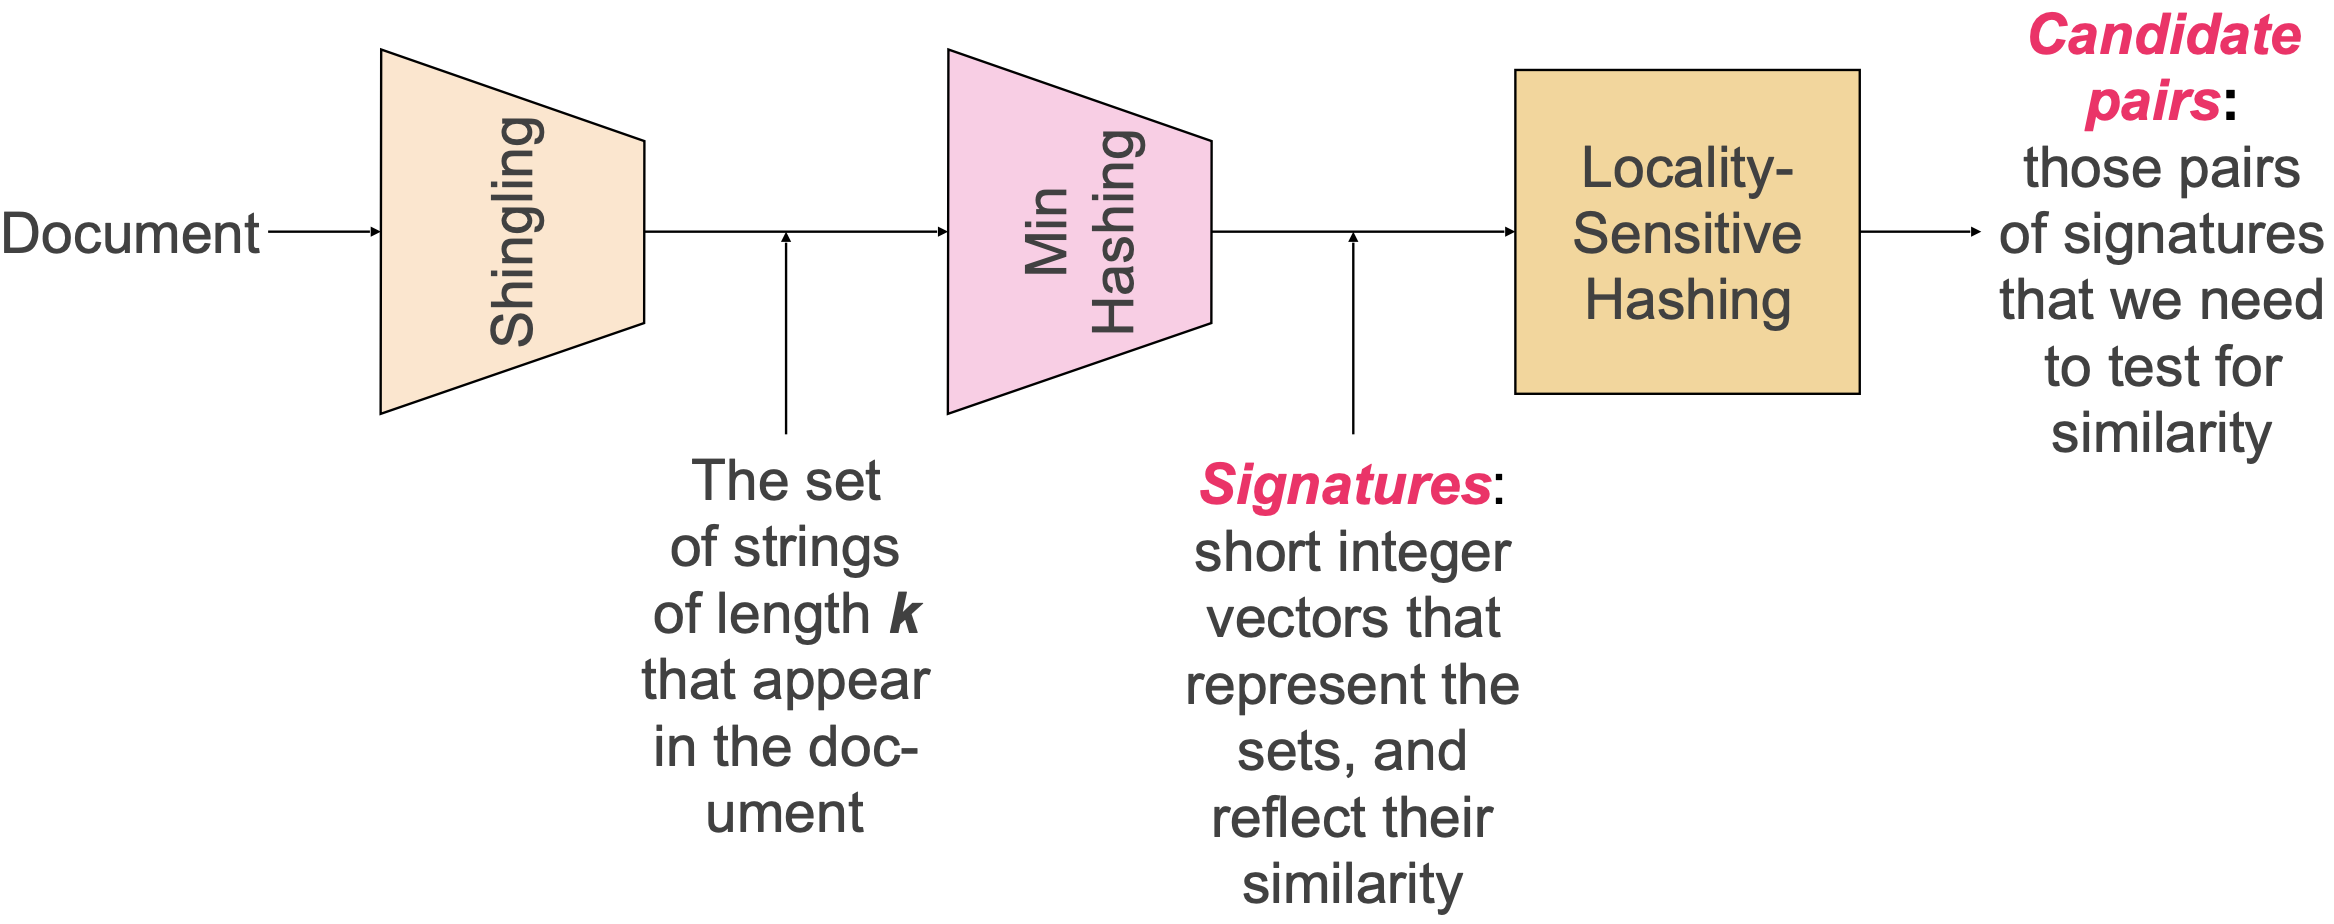
\includegraphics[scale=0.35]{figures/lsh.png}
 \caption{Locality-Sensitive Hashing}
\end{figure}


\section{LSH Steps}
\begin{enumerate}
 \item Shingling: Convert documents into sets of shingles.
 \item Min-Hashing: Convert large sets of short signatures, while preserving similarity (i.e. Jaccard similarity).
 \item Locality-Sensitive Hashing: Focus on pairs of signatures likely to be from similar documents.
\end{enumerate}
\begin{itemize}
 \item This results in candidate pairs, which are likely candidates with a high probability of being similar to the input document.
\end{itemize}

\section{Shingling}
Shingling is the process of converting documents to sets. Some simple approaches are to transform the document into sets of unique words, or "important" words.
The main problem is that the ordering of words has to be taken into account:

\subsection{Shingles}
A $k$-shingle (or $k$-gram) for a document is a sequence of $k$ tokens that appears in the document.
\begin{itemize}
 \item Tokens can be characters, words, or something else, depending on the application.
\end{itemize}

A modification of the $k$-shingle is to use shingles as a bag (multiset), and therefore counting equal sequences multiple times instead of only one.

\subsubsection{Similarity Metric for Shingles}
\begin{itemize}
 \item Document $D_i$ is a set of its $k$-shingles $C_i = S(D_i)$
 \item In this setting, each unique shingle is a dimension.
 \item The vectors will be very sparse as most documents does not contain most of the shingles.
\end{itemize}

A natural similarity measure is the \textbf{Jaccard Similarity}:

\begin{equation}
 sim(D_1, D_2) = \frac{\abs{C_1 \cap C_2}}{\abs{C_1 \cup C_2}}
\end{equation}

\subsubsection{Working Assumptions}
\begin{itemize}
 \item Documents that have lots of shingles in common have similar text, even if the text appears in different orders.
 \item $k = 5$ is ok for short documents.
 \item $k = 10$ is better for long documents.
\end{itemize}

\section{Min-Hashing}
Using pairwise Jaccard similarity directly to find near-duplicate documents would result in operations too complex and time consuming to handle. This is why min-hashing is used.

Min-hashing provides signatures (short integer vectors) that represent the sets and their similarity.

\subsubsection{Encoding Sets as Bit Vectors}
Many similarity problems can be formalized as:

Finding subsets that have a significant intersection.

\bigskip

This can be done efficiently by encoding sets using boolean vectors.

\bigskip
\begin{figure}[H]
 \centering
 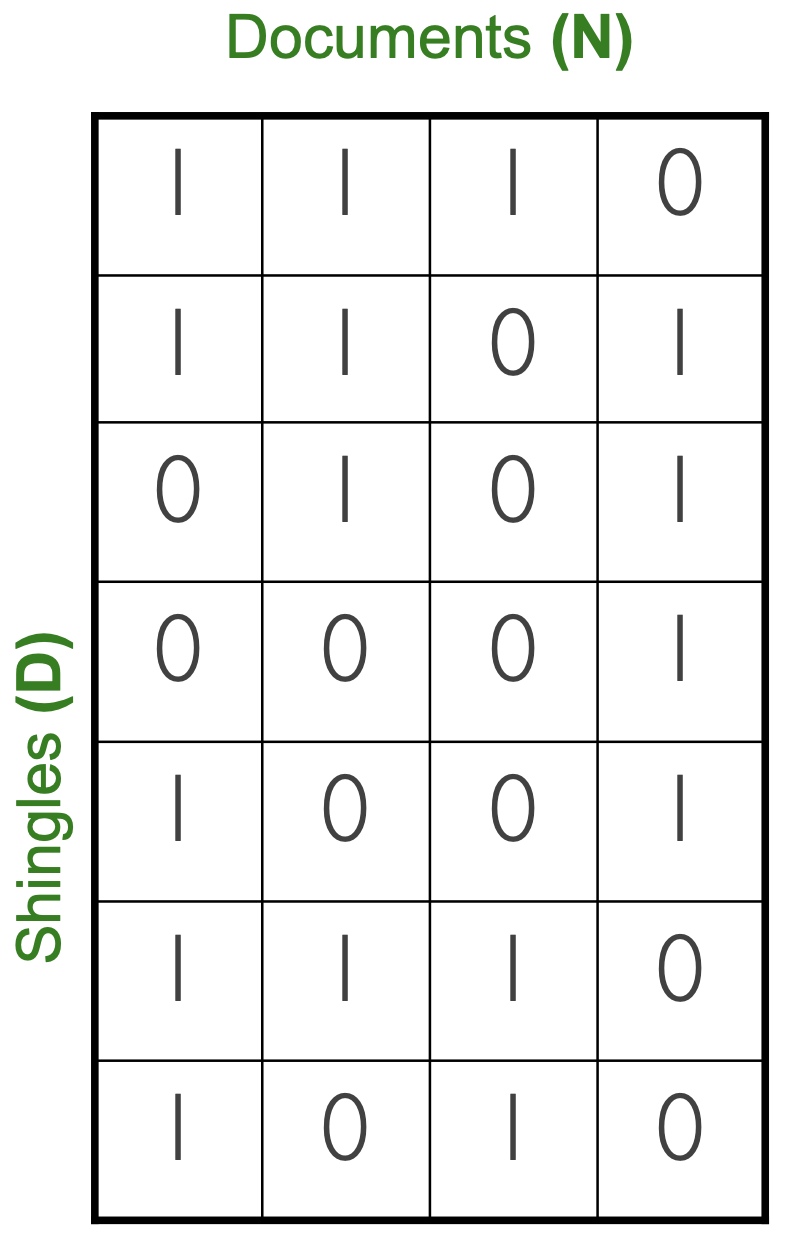
\includegraphics[scale=0.3]{figures/boolmatrix.png}

 \textit{Note:} $d(C_1, C_2) = 1 - \frac{\abs{C_1 \cap C_2}}{\abs{C_1 \cup C_2}} = 1 - \frac{3}{6}$
 \caption{Boolean Matrix}
\end{figure}

\subsection{Hashing Columns}
The key idea of hashing is to hash each column $C$ to a small signature $h(C)$ so that:
\begin{itemize}
 \item $h(C)$ is small enough to fit in the RAM.
 \item The Jaccard similarity is preserved.
\end{itemize}

The goal is to find a hash function so that if $sim(C_1, C_2)$ is high, there is a high probability that $h(C_1) = h(C_2)$, and vice versa.
The hash function places columns into a bucket, with the expected outcome being that most pairs of near-duplicate documents hash into the same bucket.

\bigskip

A suitable hash function for the Jaccard similarity is called \textbf{Min-Hashing}.

\subsection{Definition}
\begin{itemize}
 \item Imagine the rows of the boolean matrix permuted under random permutation $\pi$.
 \item Define a hash function $h_\pi(C)$ = the index of the first row in which column $C$ is $True$.
 \item Use several independent hash functions (that is, permutations) to create a signature of a column.
\end{itemize}

\begin{equation}
 \bm{h}_\pi\bm{(C)} = \bm{min}_\pi\pi\bm{(C)}
\end{equation}

Each unique combination of $1$s and $0$s can be classified as different types.

I.e. $A = 1, 1$, $B = 1, 0$, $C = 0, 1$, $D = 0, 0$.
If lower case letters denote the number of rows corresponding to the corresponding type, we get the following Jaccard similarity:
\begin{equation}
 sim(C_1, C_2) = \frac{a}{a+b+c}
\end{equation}
And the probability:
\begin{equation}
 Pr\left[h_\pi(C_1) = h_\pi(C_2)\right] = sim(C_1, C_2)
\end{equation}
And the thought-process is:

\begin{enumerate}
 \item Look down the columns $C_1$ and $C_2$ until the first $1$ appears.
 \item If the row is of type $A$, then $h(C_1) = h(C_2)$.
 \item If the row is of type $B$ or $C$, then $h(C_1) \neq h(C_2)$.
\end{enumerate}

\subsubsection{Similarity for Signatures}
\begin{itemize}
 \item The similarity of two signatures is the fraction of the hash functions in which they agree.
 \item Because of the Min-Hash property, the similarity of columns is the same as the expected similarity of their signatures.
\end{itemize}

\bigskip
\begin{figure}[H]
 \centering
 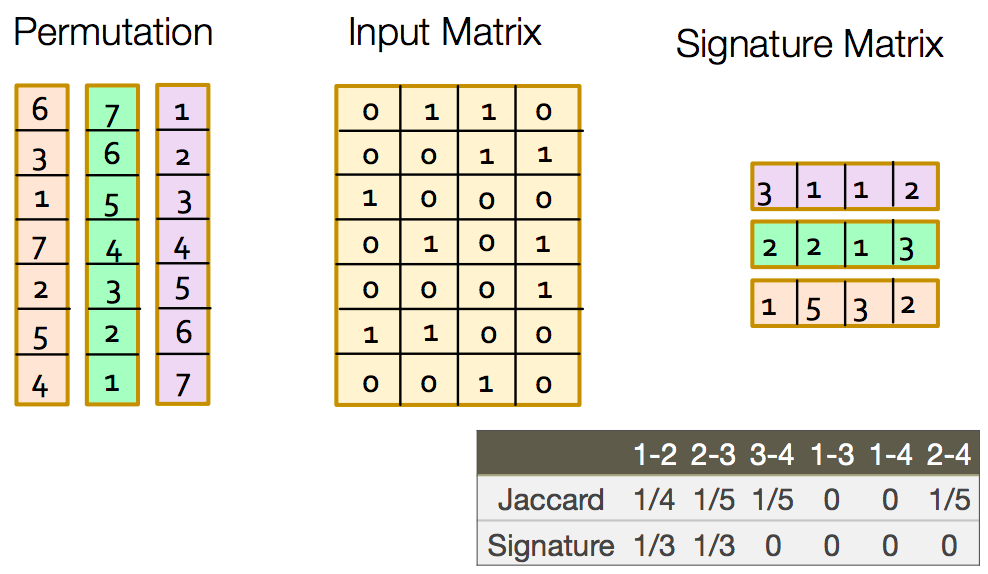
\includegraphics[scale=0.35]{figures/minhashing.png}
 \caption{Min-Hashing}
\end{figure}

\subsection{Process}
\begin{enumerate}
 \item Pick $k=100$ random permutations of the rows.
 \item Think of $\bm{sig(C)}$ as a column vector.
 \item $\bm{sig(C)[i]} = $ The index of the first row that has the value of $1$ in column $C$, given the $\bm{i}_{th}$ permutation.
 \item $\bm{sig(C)[i]} = \bm{min\left(\pi_i(C)\right)}$ 
\end{enumerate}

\section{LSH}
The goal of the locality-sensitive hashing process is to find documents with Jaccard similarity over some similarity threshold $s$.

The general idea is to use a function $f(x, y)$ that tells whether $x$ and $y$ is a candidate pair; a pair of elements whose similarity must be evaluated.

For Min-Hash matrices:
\begin{itemize}
 \item Hash columns of the signature matrix $M$ into many buckets,
 \item Each pair of documents that hashes into the same bucket is a candidate pair.
\end{itemize}

Columns $x$ and $y$ of $M$ are a candidate pair if their signatures agree on at leas the fraction $s$ of their rows.
$\bm{M}(i, x) = \bm{M}(i, y)$ for at least the fraction $s$ of $i$. It is expected that the documents $x$ and $y$ have the same Jaccard similarity as their signatures.

\bigskip

The main idea of LSH for Min-hashing is to hash columns of the signature matrix $M$ several times.
Then, arrange the columns so that only similar columns are likely to hash to the same bucket, with a high probability.
Finally, the candidate pairs are those columns that hash to the same bucket.

\subsection{Process of LSH}
\begin{enumerate}
 \item Divide matrix $M$ into $b$ bands of $r$ rows.
 \item For each band, hash its portion of each column to a hash table with $k$ buckets, while making $k$ as large as possible.
 \item The candidate column pairs are those bands that hash to the same bucket for more than one band.
 \item Tune $b$ and $r$ to catch most similar pairs, and minimize the number of non-similar pairs.
\end{enumerate}

\subsubsection{Simplified Assumptions}
\begin{itemize}
 \item There are enough buckets that columns are unlikely to hash to the same bucket unless they are identical in a particular band.
 \item It is assumed that all bands in the bucket are identical.
 \item These assumptions are only needed to simplify the analysis, not for the correctness of the algorithm.
\end{itemize}

\subsubsection{Some Probabilities}
Given the columns $C_1$ and $C_2$ with the similarity $s$, and that $b$ bands with $r$ rows is selected:
\begin{itemize}
 \item The probability that all rows in the band are equal $ = s^r$
 \item The probability that some rows in the band are unequal $ = 1 - s^r$
 \item The probability that no bands are identical after $b$ bands $ = (1-s^r)^b$
 \item The probability that at least one band is identical after $b$ bands $ = 1 - (1-s^r)^b$
\end{itemize}

\subsection{LSH Decisions}
Some parameters have to be adjusted to balance the false positives and negatives and get the most desired result when using LSH. This includes:
\begin{itemize}
 \item The number of Min-Hashes (rows of $M$).
 \item The number of bands $b$.
 \item The number of rows $r$ per band.
\end{itemize}

\subsection{Summary}
\begin{itemize}
 \item Tune $M$, $b$, and $r$ to get almost all pairs with similar signatures, but eliminate most pairs that do not have similar signatures.
 \item Check in the main memory that candidate pairs do have similar signatures.
 \item Optional: In another pass through the data, check that the remaining candidate pairs represent similar documents.
\end{itemize}


\chapter{Dimensionality reduction}
\section{Dimensionality Reduction}
The purpose of dimensionality reduction is to:
\begin{itemize}
    \item Avoid curse of dimensionality.
    \item Reduce the amount of time and memory required by data mining algorithms.
    \item Allow data to be more easily visualized.
    \item May help to eliminate irrelevant features or reduce noise.
    \item Recommender systems
\end{itemize}
Some of the techniques used for dimensionality reduction are:
\begin{itemize}
    \item Principle Component Analysis
    \item Singular Value Decomposition
\end{itemize}

This is done by searching for a plane with a lower count of dimensions, which approximately fits the data values.

\subsubsection{Data compression}
By compressing the data, data mining algorithms can be trained faster. Besides, redundant data such as equal measures, but in different units, could be compressed/merged.

\subsubsection{Visualization}
Dimensionality reduction can improve how we display information in a tractable manner for human consumption.
This is important because visually understandable information often helps to develop algorithms.

\section{Singular Value Decomposition (SVD)}
\begin{theo}[SVD]{theo:theo80}
\label{eq:SVD}
\[
A_{[m \cdot n]} = U_{[m \cdot r]} \Sigma_{[r \cdot r]} V_{[n \cdot r]}^T
\]
\end{theo}
Where:
\[
    \begin{aligned}
        & A = \text{Input data matrix} \\
        & \text{I.E m documents, n terms}
        \\
        \\
        & U = \text{Left Singular vectors} \\
        & \text{I.E m documents, r concepts}
        \\
        \\
        & \Sigma = \text{Singular values} \\
        & \text{r - rank of matrix } A
        \\
        \\
        & V = \text{Right Singular vectors} \\
        & \text{I.E n terms, r concepts}
    \end{aligned}
\]

\bigskip
\begin{figure}[H]
\centering
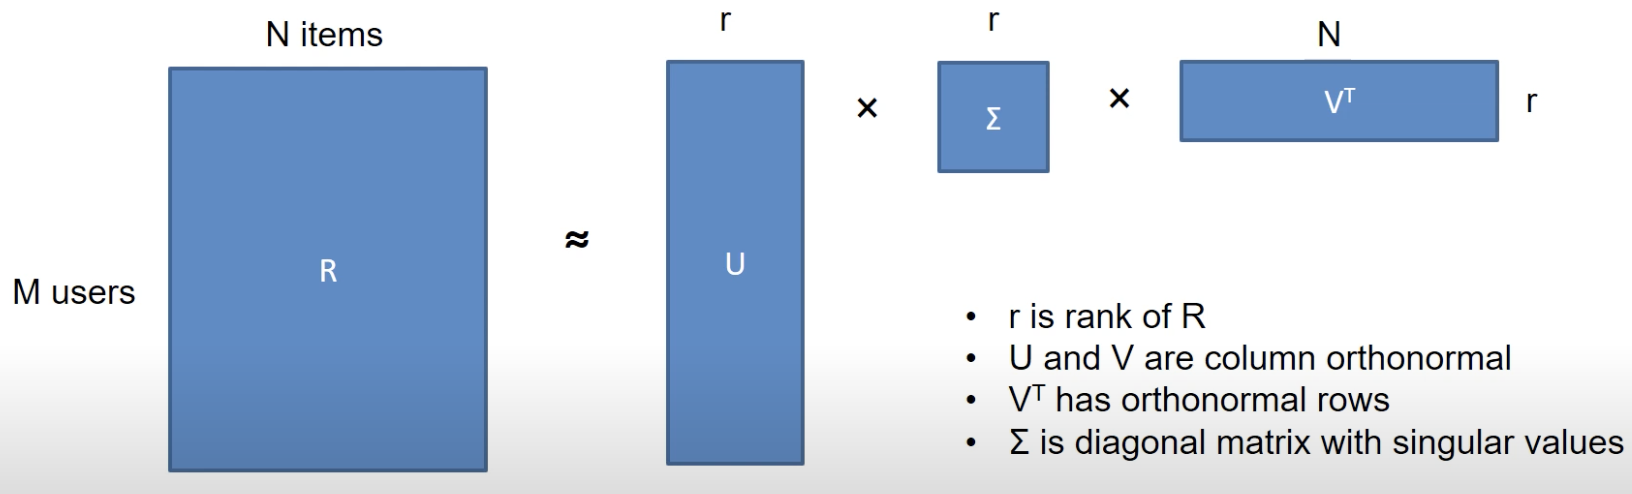
\includegraphics[scale=0.5]{figures/svd.png}
\caption{Single Value Decomposition}
\end{figure}

For information on how to compute the singular value decomposition (with examples), visit: 
\href{http://web.mit.edu/course/other/be.400/OldFiles/www/SVD/Singular_Value_Decomposition.htm}{Singular Value Decomposition (SVD) tutorial}.


\section{Principal Component Analysis (PCA)}
PCA is the most commonly used dimensionality reduction method.

\subsection{Goal}
The goal of the PCA is to find a single line (or plane in higher dimensions) onto which to project the input data.

The line/plane can be found by finding a lower-dimensional surface so the sum of squares onto that surface is minimized.

\subsection{General Case}
\begin{itemize}
    \item Given an $m * n$ matrix, the goal is to find an $m * k$ matrix.
    \item Find a set of vectors which we project the data onto the linear subspace spanned by that set of vectors.
    \item We can define a point in a plane with $k$ dimensional vectors.
\end{itemize}

\subsection{Algorithm}
The PCA Algorithm requires some preprocessing to work properly.
\begin{itemize}
    \item Step 1: Preprocessing
    \begin{itemize}
        \item Mean normalization - Replace each $x_{ji}$ with $x_{ji}$-$\mu_{j}$, subtract the mean from the value, so the mean is re-scaled to be 0.
        \item Feature scaling (dependent on data) - If the features have very different scales, normalize them by changing $x_{ji}$ to $\frac{x_{ij}-\mu_{j}}{s_{j}}$, where $s_{j}$ is some measure of the range, i.e. $max$, $min$, or $standard$ $deviation$.
    \end{itemize}
    \item Step 2: Compute the covariance matrix
    \begin{itemize}
        \item $COV(x, y) = \frac{1}{n-1}\sum_{i=1}^n(x_i-\hat{x})(y_i-\hat{y})$
        \item This results in an $\left[n*n\right]$ matrix.
        \item $x_i$ and $y_i$ are $\left[m*1\right]$ vectors.
    \end{itemize}
    \item Step 3: SVD
    \begin{itemize}
        \item Compute the SVD on the covariance matrix C.
        \item $\left[U, \Sigma, V^T\right] = SVD(C)$
        \item The U matrix is an $\left[n*r\right]$ matrix.
        \item To reduce the system from $n$-dimensions to $k$-dimensions, take the first $k$ vectors from $U$ (The first $k$ columns).
    \end{itemize}
\end{itemize}
\subsection{Transformation}
To change $X$ (which is $n$ dimensional) to $z$ (which is $k$ dimensional):
\begin{enumerate}
    \item Take the first $k$ columns of the $U$ matrix and stack in columns. This gives the $n*k$ matrix $U_{Reduced}$.
    \item Calculate $z$: $z = U_{Reduced}^T * X$
    \item $\left[[k*n]\right]*\left[[n*1]\right]$
    \item This generates a matrix which is $k*1$ per data row.
\end{enumerate}

\subsection{Meassure Quality of PCA}
To meassure how good the implemented PCA is, we can meassure the reconstruction error:
\begin{itemize}
    \item Given the reduced data $U_{Reduced}$ in $K$ dimensions .
    \item $X_{Approx}=U_{Reduce}*Z$ 
\end{itemize}
\begin{equation}
    \frac{\frac{1}{m}\sum_{i=1}^m\norm{x_i-x_i^{approx}}^2}{\frac{1}{m}\sum_{i=1}^m\norm{x_i}^2} \leq 0.01
\end{equation}

\subsection{Choosing the Parameter k}
We want to choose the $k$ value which results in the smallest ratio between the averaged squared projection error with the total variation in the data.
This makes sense, as we want $x_i \approx x_i^{Approx}$ to retain as much information as possible.


\chapter{Advanced Classifiers (Naive Bayes)}
\section{Probability theory recap}
Probability theory is a branch of mathematics concerning numerical descriptions
of how likely an event is to occur. Formalised by Andrey Kolmogorov in 1933.
\cite{kolmogorov1960foundations} He formalised the modern interpretation of 
probability theory. The axioms from this publication is:

\medskip

\textbf{The First Axiom}: The Probability of an event $E$ is a non-negative real
number.

\begin{equation}
    P(E) \in \mathbb{R}, P(E) \geq 0, \quad \forall E \in F 
\end{equation}

where $F$ is the event space.

\medskip

\textbf{The Second Axiom}: The Probability of at least one element occuring in
the sample space is $1$

\begin{equation}
    P(\Omega) = 1
\end{equation}

\medskip

\textbf{The Third Axiom}: The probability of the union of disjoint sets is equal
to the sum of the probabilities of the disjoint sets.

\begin{equation}
    P\left(\bigcup_{i = 1}^{\infty} E_i \right) = \sum_{i = 1}^{\infty} P(E_i)
\end{equation}

\section{Conditional Probability Recap}

\begin{equation*}
P(A \mid B) = \frac{P(A \cap  B)}{P(B)}
\end{equation*}

This is read as: Probability of event A given B. 

\section{Bayes Theorem}

Bayes theorem is derived from the definition of codnitional 
probability. Given that

\begin{equation*}
    P(A \cap B) = P(B \cap A)
\end{equation*}

Since the intersection operator does not care about order. We can rearrange
equation and get

\begin{equation*}
    P(A \cap B) = P(A \mid B)P(B) = P(B \mid A)P(A)
\end{equation*}

and we can substitute $P(A \cap B)$ with the equation above and get:

\begin{theo}[]{theo:theo91}
\label{eq:bayes}
\[
P(A \mid B) = \frac{P(B \mid A) P(A)}{P(B)}
\]
\end{theo}

\section{Bayes Theorem for Continuous Values}

We need to assume that the values we are interested in have a Gaussian distribution.
\begin{itemize}
    \item Find the mean $\mu$
    \item Find the variance $\sigma^2$
    \item Use the Gaussian distribution to calculate the probability $P(A)$
\end{itemize}
\medskip

For conditional probabilities:
\begin{itemize}
    \item Find the mean $\mu_B$ for only the condition $B$
    \item Find the variance $\sigma^2_B$ for only the condition $B$
    \item Use the Gaussian distribution to calculate the conditional probability $P(A|B)$
\end{itemize}
\medskip

For inequalities, we need to integrate the Gaussian density (preferably by computing the standard Gaussian density first).

\section{Bayesian Classifiers}
\subsection{Goal}
Given a record with attributes $(A_1, A_2, \cdots, A_n)$, the goal of the bayesian classifier is th predict the class $C$.
Specifically, we want the classifier to fint the value of $C$ that maximizes $P(C|A_1, A_2, \cdots, A_n)$.

\subsection{Approach}
\begin{enumerate}
    \item Compute the posterior probability for all values of $C$ based on Bayes theorem.
    \item Choose the value of $C$ that maximizes the posterior probability.
    \begin{itemize}
        \item This is equivalent to choosing the value of $C$ \\ that maximizes $P(A_1, A_2, \cdots, A_n | C) P(C)$, \\ because the denominators are equal
    \end{itemize}
\end{enumerate}
\medskip

Computing $P(A_1, A_2, \cdots, A_n | C) P(C)$ is done as such:
\begin{enumerate}
    \item Assume independence among attributes $A_i$ when the class is given:
    \begin{itemize}
        \item $P(A_1, A_2, \cdots, A_n | C) = P(A_1|C_j) P(A_2|C_j) \cdots P(A_n|C_j)$ 
    \end{itemize}
    \item Estimate $P(A_i|C_j)$ for all $A_i$ and $C_j$
    \item The new point is classified to $C_j$ if $P(C_j)\prod P(A_i|C_j)$ is maximal
\end{enumerate}

\subsection{Estimating Probabilities from Data}
For continuous attributes:
\begin{enumerate}
    \item Discretize the range into bins:
    \begin{itemize}
        \item One ordinal attribute per bin
        \item Violates independence assumption
    \end{itemize}
    \item Two-way split
    \begin{itemize}
        \item Choose only one of the two splits as a new attribute
    \end{itemize}
    \item Probability density estimation
    \begin{itemize}
        \item Assume that the attribute follows a normal distribution
        \item Estimate the mean and the variance
        \item Estimate the conditional probability $P(A_i|C)$ from the known distribution
    \end{itemize}
\end{enumerate}

\bigskip
\begin{figure}[H]
\centering
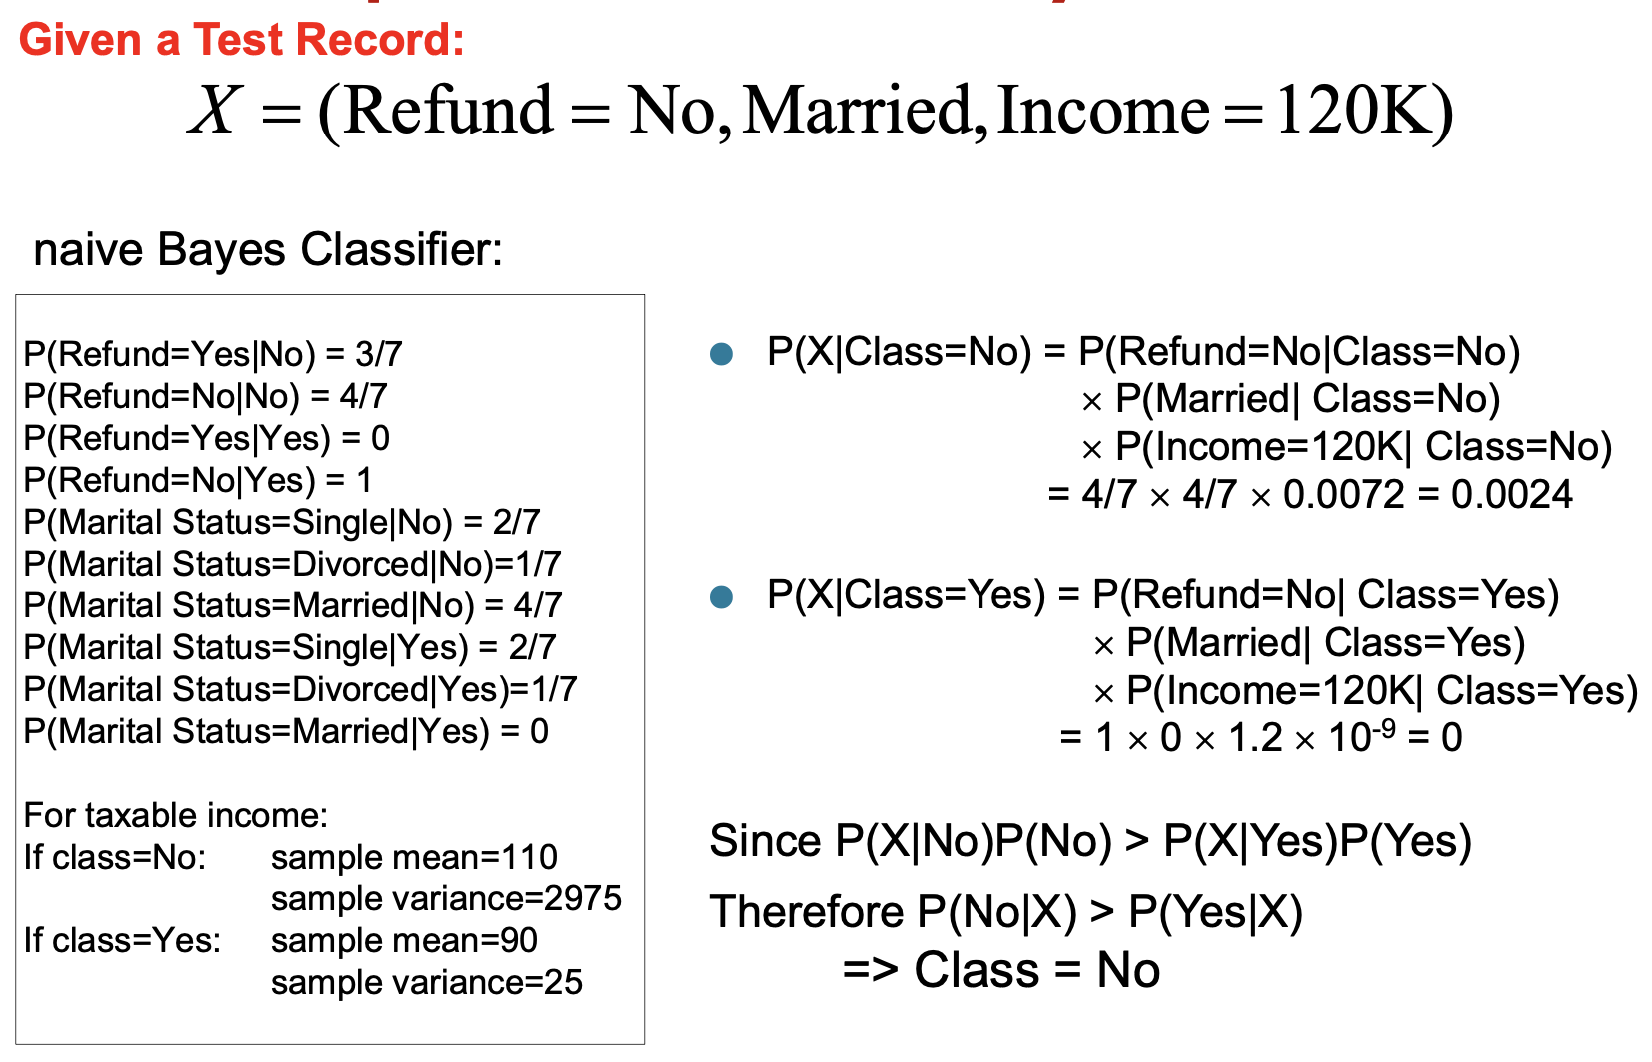
\includegraphics[scale=0.4]{figures/prob_est_data.png}
\caption{Example of deciding class}
\end{figure}

\subsection{Naive Bayes Classifier problems}
In the previous figure, one of the conditional probabilities is zero, meaning that the entire expression becomes zero.
This is often an effect of having an incomplete training set. This means that the class, given the conditional probability, will never be chosen.

This can be "fixed" by using some type of smoothing:
\begin{itemize}
    \item Original: $P(A_i|C) = \frac{N_{ic}}{N_c}$
    \item Laplace: $P(A_i|C) = \frac{N_{ic}+1}{N_c+c}$
    \item m-estimate: $P(A_i|C) = \frac{N_{ic}+mp}{N_c+m}$
\end{itemize}

Where $c =$ number of classes, $p =$ prior probability, and $m =$ own parameter.

\section{Bayesian Belief Network (BBN)}
\begin{itemize}
    \item Conditional independence assumption is not always practical.
    \item A Bayesian belief network provides a graphical representation of dependencies.
    \begin{itemize}
        \item A directed acyclic graph (dag) encoding the dependence relationships among a set of variables.
        \item A probability table associating each node to its immediate parent node.
    \end{itemize}
    \item Calculating the probability of a variable, which is dependent on some other variables, can often be simplified to only depend on the direct parent(s).
\end{itemize}

\section{Summary of Naive Bayes}
\begin{itemize}
    \item Robust to isolated noise points.
    \item Handle missing values by ignoring the instance during probability estimate calculations.
    \item Robust to irrelevant attributes.
    \item Independence assumption may not hold for some attributes.
    \begin{itemize}
        \item Use other techniques such as Bayesian Belief Networks (BBN).
    \end{itemize}
\end{itemize}


\chapter{Advanced Classifiers (Linear Regression)}
\section{Notation}
\begin{itemize}
    \item $m = $ The number of training examples
    \item $x = $ The input variables / features
    \item $y = $ The output variable/"target" variables
    \item $(x_i, y_i) = $ A specific example ($i_{th}$ training example)
\end{itemize}

Passing the features into a learning algorithm that outputs a function (denoted $h = $ hypothesis), resulting in the function:
\[
    h_\theta(x) = \theta_0+\theta_1 x
\]
where $\theta_i$ are parameters, $\theta_0$ is the zero condition, and $\theta_1$ is the gradient.

\section{Cost Function}
A cost function lets us figure out how to fit the best straight line to our data.
We want to solve a minimization problem where we minimize $(h_\theta(x)-y)^2$.

The most common cost function is the mean squared error (MSE):
\[
    J(\theta_0, \theta_1) = \frac{1}{m}\sum_{i=1}^m\left(h_\theta(x_i)-y_i\right)^2
\]

Note that multiplying the cost function by $\frac{1}{2}$ does not change the location of the minima, which is why we use it to form the following cost function:
\bigskip

One half mean squared error:
\[
    J(\theta_0, \theta_1) = \frac{1}{2m}\sum_{i=1}^m\left(h_\theta(x_i)-y_i\right)^2
\]

The cost function determines the parameters, and the values associated with the parameters determine how the hypothesis behaves.
Different values generate different hypotheses.

The MSE cost function is convex.

Finding the global minima in linear regression can be done with a gradient descent algorithm.

\subsection{Cost Function for Multiple Variables}
\[
    J(\theta_0, \theta_1, \cdots, \theta_n) = \frac{1}{2m}\sum_{i=1}^m\left(h_\theta(x_i)-y_i\right)^2
\]

\section{Batch Gradient Descent Algorithm (BGD)}
\begin{itemize}
    \item In each step you look at all the training data
\end{itemize}

\subsubsection{Progress}
\begin{enumerate}
    \item Start with initial guesses, i.e. $(0, 0)$
    \item Keep changing $\theta_0$ and $\theta_1$ a little bit to reduct $J(\theta_0, \theta_1)$
    \item Each time the parameters change, select the gradient which reduces $J(\theta_0, \theta_1)$ the most
    \item Repeat until we converge to a local/global minima
\end{enumerate}
Different starting points will often result in different minimas.

\subsubsection{Formal progress}
\begin{itemize}
    \item Do the following until convergence:
    \begin{itemize}
        \item $\theta_j:=\theta_j-\alpha\frac{\partial}{\partial\theta_j}J(\theta_0, \theta_1)$
        \item For $j=0$ and $j=1$ in this example.
    \end{itemize}
    \item $\alpha$ is the learning rate
    \item $\alpha$ controls how aggressive the gradient descent is
\end{itemize}

"For $j=0$ and $j=1$" means that we update both parameters simultaneously. This is done by first solving the derivative for $\theta_0$ and storing it in a temporary variable. Do the same for $\theta_1$, and then update the original $\theta_j$-values.

\subsubsection{Partial Derivatives}
\[
    \frac{\partial}{\partial \theta_j}J(\theta_0, \theta_1) = \frac{\partial}{\partial\theta_j}\frac{1}{2m}\sum_{i=1}^m(\theta_0+\theta_1x_i-y_i)^2
\]
\[
    \frac{\partial}{\partial \theta_0}J(\theta_0, \theta_1) = \frac{1}{m}\sum_{i=1}^m(\theta_0+\theta_1x_i-y_i)*1
\]
\[
    \frac{\partial}{\partial \theta_1}J(\theta_0, \theta_1) = \frac{1}{m}\sum_{i=1}^m(\theta_0+\theta_1x_i-y_i)x_i^{(1)}
\]
\[
    \frac{\partial}{\partial \theta_j}J(\theta_0, \cdots, \theta_n) = \frac{1}{m}\sum_{i=1}^m(\theta_0+\cdots+\theta_nx_i-y_i)x_i^{(j)}
\]

\subsection{Gradient Descent in Practice}
\begin{itemize}
    \item Feature Scaling (normalize)
    \begin{itemize}
        \item Problems with multiple features should be scaled to a more even scale across the features.
        \item One common way is to use the mean to scale all data into the range $\left[-1, 1\right]$.
        \item Try to create a range between $\left[-3, 3\right]$ and $\left[-\frac{1}{3}, \frac{1}{3}\right]$.
        \item This is done by $x_i = \frac{x_i-\hat{x}}{max(x)-min(x)}$
    \end{itemize}
    \item Running gradient descent on this kind of cost function can take a long time to find the global minima.
\end{itemize}

\section{Practical Tips}
\begin{itemize}
    \item Plot $min(J(\theta))$ with the number of iterations to clearly illustrate the convergence.
    \item Start with a low learning rate, and gradually increase it. It is normal to go for roughly treefold increments (multiply by 3).
    \item We could also use a polynomial regression on the form $(\theta_0 + \theta_1x + \theta_2x^2)$.
\end{itemize}


\chapter{Advanced Classifiers (Logistic Regression)}
\section{The Logistic Classifier}
The logistic regression model is a binary classification problem.
Linear regression for binary classification is not a viable option as the 
decision boundary will not separate the two categories correctly because of 
the nature of the mean square error.
The classifier should output either $1$ or $0$, depending on the data.
Where the classifier outputs the probability of the class given the 
observations. The problem is that a regression model has a domain of $(-\infty, \infty)$
and we want to somehow map this to the probability of observing a class which
has the domain $(0, 1)$. To do this we introduce odds:

\begin{equation*}
    \text{odds} = \frac{p}{1 - p}
\end{equation*}

The odds is the ratio of successes to failures. Colloquially we talk about odds
all the time. Statements like \textit{For every 4 people 1 are...}. This is in
an odds of $4:1$ or just $4$. The probability on the other hand for the same
statement is \textit{1 out of 5 are...} or 
\textit{There is a one in fifth chance of...}. 
Odds have the domain of $(0, \infty)$, which is closer to that of a regression
model but still not quite there. Taking the log of the odds 

\begin{equation*}
    \ell  = \log_{b} \frac{p}{1 - p}
\end{equation*}

we map the odds to the domain $(-\infty, \infty)$. Now, we assume a linear 
relationship between the feature and the log-odds

\begin{equation*}
    \ell  = \log_{b} \frac{p}{1 - p} = \theta^T x
\end{equation*}

And we can now recover the odds by exponentiation the log odds

\begin{equation*}
    \frac{p}{1 - p} = b^{\theta^T x}
\end{equation*}

And by algebraic manipulation we get

\begin{equation*}
    p = \frac{1}{1 + b^{-\theta^T x}}
\end{equation*}


In most litterature, the classification hypothesis representation used for
logistic regression uses $b = e$:

\[
    h_\theta(x) = g(\theta^Tx) = \frac{1}{1+e^{-\theta^Tx}}
\]
\bigskip

This is the sigmoid function (the logistic function).

The function is used as such:

\begin{equation}
    \left\{\begin{matrix}
        1 & \text{if } h_\theta(x) > 0.5 \\ 
        0 & \text{otherwise}
        \end{matrix}\right.
\end{equation}

\subsection{Logistic Classifier for Higher-Order Terms}
As in polynomial regression, the logistic classifier can be used for higher order terms by adding higher order terms. I.e. $g(\theta_0 + \theta_1x_1+\theta_3x_1^2+\theta_4x_2^2)$

\section{Problems with the Linear Regression Cost Function}
The mean square error function results in a convex PDF when given it is given linear values. This is not the case for logistic regression. This means that the MSE would most likely only find a local minimum, not a global one.

\section{Logistic Regresssion Cost Function}
\begin{equation}
    Cost(h_\theta(x), y) = 
    \left\{\begin{matrix}
        -ln(h_\theta(x)) & \text{if } y=1 \\ 
        -ln(1-h_\theta(x)) & \text{if } y=0
        \end{matrix}\right.
\end{equation}

This can be rewritten into a single function:

\begin{equation}
    Cost(h_\theta(x), y) = -y ln(h_\theta(x)) - (1-y)ln(1-h_\theta(x))
\end{equation}

\section{Process}
The process forwards is the same as in the linear regression chapter.

\section{Multiclass Classifier for Logistic Regression}
Extending the logistic regression from a binary classifier to a multiclass classifier can be done in a "one vs. all" classification.

This means that the algorithm is conducted multiple times, each time changing which class is the positive class (where all the other classes are negative).


\chapter{Classification (Regularization)}
\section{Addressing Overfitting}
Multiple strategies can be used to check if overfitting occurs:
\begin{itemize}
    \item Plot the hypothesis to check for overfitting. Might not always work.
    \item Reduce the number of features
    \item Regularization
\end{itemize}

\section{Regularization}

Regularization is the process of adding information in order to solve an 
ill-posed problem or to prevent overfitting. Normally in machine learning
regularization is done by introducing a regularization term $R(f)$ to the loss
function 

\begin{equation*}
    \min_f \sum_{i = 1}^n V(f(x_i), y_i) + \lambda R(f)
\end{equation*}

Where $V$ is the underlying loss function and $R(f)$ is typically chosen to 
impose a penalty on the complexity of $f$. Regularization in one way imposes
occam's razor on the solution, the principle that the simpler explanation 
(model) is usually the best. Another perspective is the Bayesian one where 
prior knowledge is applied to the model parameters.

\begin{itemize}
    \item Small values for parameters correspond to a simpler hypothesis (you effectively get rid of some of the terms).
    \item A simpler hypothesis is less prone to overfitting.
\end{itemize}

\subsection{Cost function optimalization}
We can penalize some of the higher-order $\theta$ parameters and make them very small:

\[
    \min\frac{1}{2m}\sum_{i=1}^{m}\left(h_{\theta}(x_i)-y_i\right)^2 + 1000\theta_3^2 + 1000\theta_4^2
\]

\subsection{Regularization on features}
Unlike in a polynomial, we don't know which parameters are the high-order terms. The solution for this is to penalize all the parameters.

By convention, we don't penalize $\theta_0$, but all other parameters, with the regularization parameter $\lambda$.

\[
    J(\theta) = \frac{1}{2m}\left[\sum_{i=1}^{m}\left(h_{\theta}(x_i)-y_i\right)^2 + \lambda\sum_{j=1}^{n}\theta_j^2\right]
\]

\subsection{Regularized Gradient Descent}
\[
    \theta_j := \theta_j - \alpha\left[\frac{1}{m}\sum_{i=1}^{m}\left(h_{\theta}(x_i)-y_i\right)x_i^{(j)} + \frac{\lambda}{m}\theta_j\right]
\]

\[
    \theta_j := \theta_j\left(1-\alpha\frac{\lambda}{m}\right) - \alpha\frac{1}{m}\sum_{i=1}^{m}\left(h_{\theta}(x_i)-y_i\right)x_i^{(j)}
\]

Given a typical small learning rate $\lambda$ and a large number of terms $m$, we see that $\theta_j$ is multiplied by a value close to $1$ (around $0.95-0.99$).


% \chapter{Neural Network Computations}
\chapter{Deep Learning (Neural Network)}
\section{Achievements of Deep Learning}
Deep Learning has had an explosion in applications and research and development
for the last decade. These applications include:

\begin{itemize}
    \item Automatic speech recognition
    \item Image recognition
    \item Visual art processing
    \item Natural language processing
    \item Drug discovery and toxicology
    \item Customer relationship management
    \item Recommendation systems
    \item Bioinformatics
\end{itemize}

The theoretical foundations of the field is old (mid 19th century), but the 
playground for these algorithms has just now arrived. These include large
datasets, computational hardware and software. 

\section{Comparison with traditional machine learning}
In traditional machine learning development. One needs domain knowledge for
developing good models. Domain knowledge let's you select good features 
and good features give good models. One example could be a certain visual
feature in a certain kind of biomedical image. This field is called 
\textbf{feature engineering}. 

\section{Feature Learning}
Feature Learning, also known as \textbf{Representation Learning} is a set of
techniques that allow systems to automatically discover the representation 
needed for feature detection or classification. Feature learning methods 
let us replace the manual feature engineering that is done in traditional 
machine learning development. A lot of deep learning architectures for 
representation learning have been researched and published in the last decade.

\section{Motivations for deep learning}

Deep Learning let's us model nonlinear decision boundaries by introducing
nonlinearities in the activation functions and deep architectures. This means 
that deep learning is especially fit for problems that are too complex for 
linear methods. One could question wether models like logistic regression could
be used with polynomial decision boundaries to achieve the same thing. 
The problem with using regression is that it achieves this by introducing
polynomial features. The number of features the model must take into account
is then 

\begin{equation*}
    O(n^b)
\end{equation*}

where $b$ is the polynomial degree that you want the model to incorporate. 
For $100$ features, introducing $b = 2$ gives over 5000 features. This is not
feasible. 

\section{Artificial Neuron}
\begin{itemize}
    \item Feed input via input nodes
    \item Logistic unit does some computation
    \item Sends output
\end{itemize}

\bigskip
\begin{figure}[H]
\centering
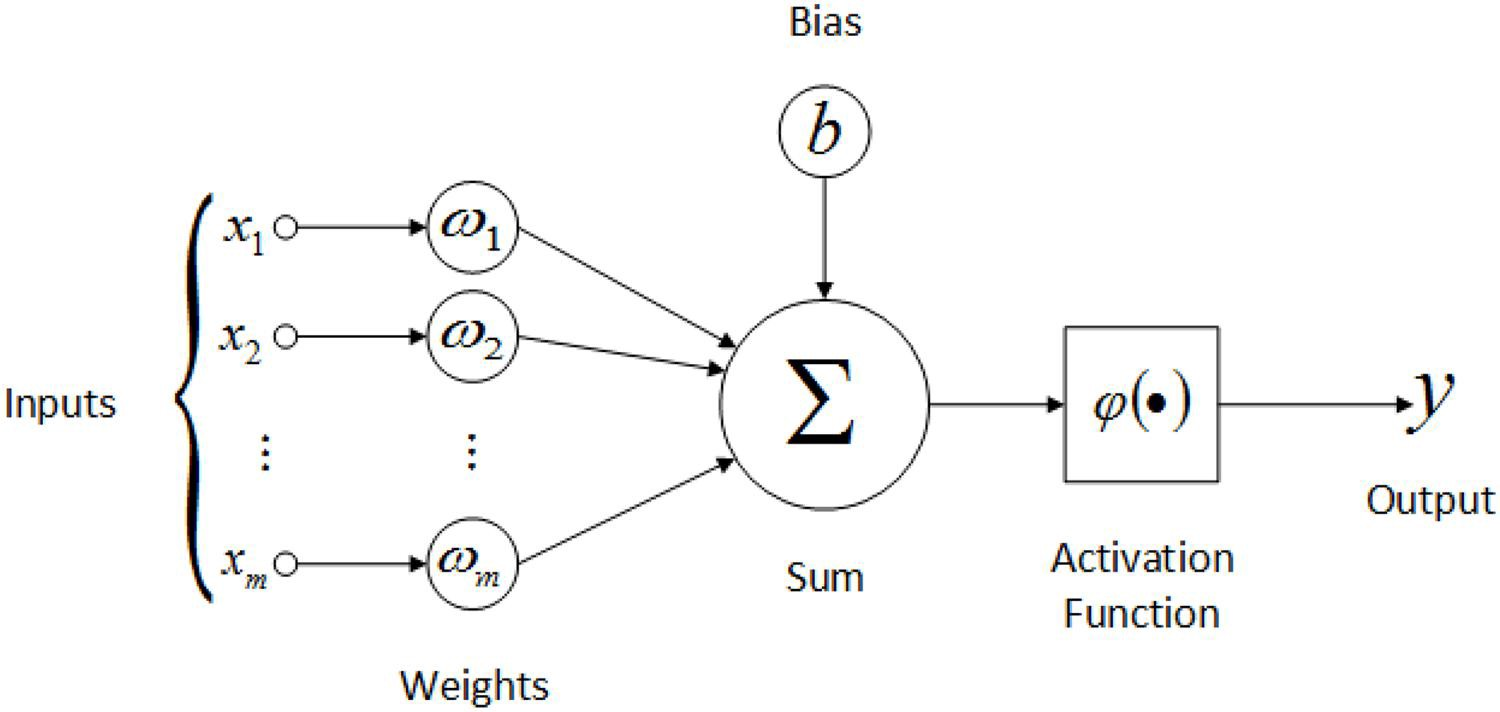
\includegraphics[scale=0.25]{figures/artificialneuron.jpeg}
\caption{Artificial Neuron}
\end{figure}

The activation function is typically the sigmoid function, a hyperbolic tangent, 
or a rectified linear unit (ReLU). They must be a non-linear function because
several layers of linear activation functions still yield a linear decision 
boundary. Deep layers of non-linear activations yield complex decision
boundaries.

\section{Notations}
\begin{itemize}
    \item $a_i^{(j)}$ - Activation of unit $i$ in layer $j$ (the output of the node)
    \item $\theta^{(j)}$ - Matrix of parameters (controlling the activation from one layer to the next)
    \item $g(\theta^Tx)$ - The activation function
\end{itemize}

\section{Multiclass Classification}
\begin{itemize}
    \item Given $N$ classes:
    \begin{itemize}
        \item Build a neural network with $N$ output units
        \item Use one-hot encoding to encode the output as an array of $N-1$ zeros and one $1$.
    \end{itemize}
\end{itemize}

\section{Cost function for Neural Networks}
The cost function can generate $k$ outputs, meaning that the sigmoid function (or any other cost functions) returns a $k$ dimensional vector.

The cost function is combined by two parts.

\bigskip

The first part finds the mean of the sum of each training sample $m$, over the sum of each class $k$. All classes has a "one-vs-all" comparison. This gives the following expression:

\[
    -\frac{1}{m}\left[\sum_{i=1}^m\sum_{k=1}^Ky_k^{(i)} \log\left(h_\Theta(x^{(i)})\right)_k+(1-y_k^{(i)}) \log\left(1-(h_\Theta(x^{(i)}))_k\right)\right]
\]

The second part is the regularization term. In this part, we sum all layers $L-1$, over all units in each layer $s_t$, over all the input layers $j$:

\[
    \frac{\lambda}{2m}\sum_{l=1}^{L-1}\sum_{i=1}^{s_t}\sum_{j=1}^{s_l+1}(\Theta_{ji}^{(l)})^2
\]

\section{Learn this better...}

% 31.30

% \bigskip
% \begin{figure}[H]
% \centering
% \includegraphics[scale=0.5]{figures/}
% \caption{}
% \end{figure}

% \begin{theo}[]{theo:theo}
% \label{eq:}
% \[
% a
% \]
% \end{theo}
%
% \section{}

\bibliography{references}

\end{document}
